% ============================================================
% ============================================================
%  ICE ACCRETION
% ============================================================
% ============================================================

\section[Ice Accretion]{\textbf{Ice Accretion}}


% ============================================================
%  Ice Mass Grid Convergence
% ============================================================

\begin{frame}{\small  Ice Mass Grid Convergence (15 Bins)}
\scriptsize
\vspace{-0.15cm}
\begin{columns}[T,onlytextwidth]

\begin{column}{0.50\textwidth}
    \centering
    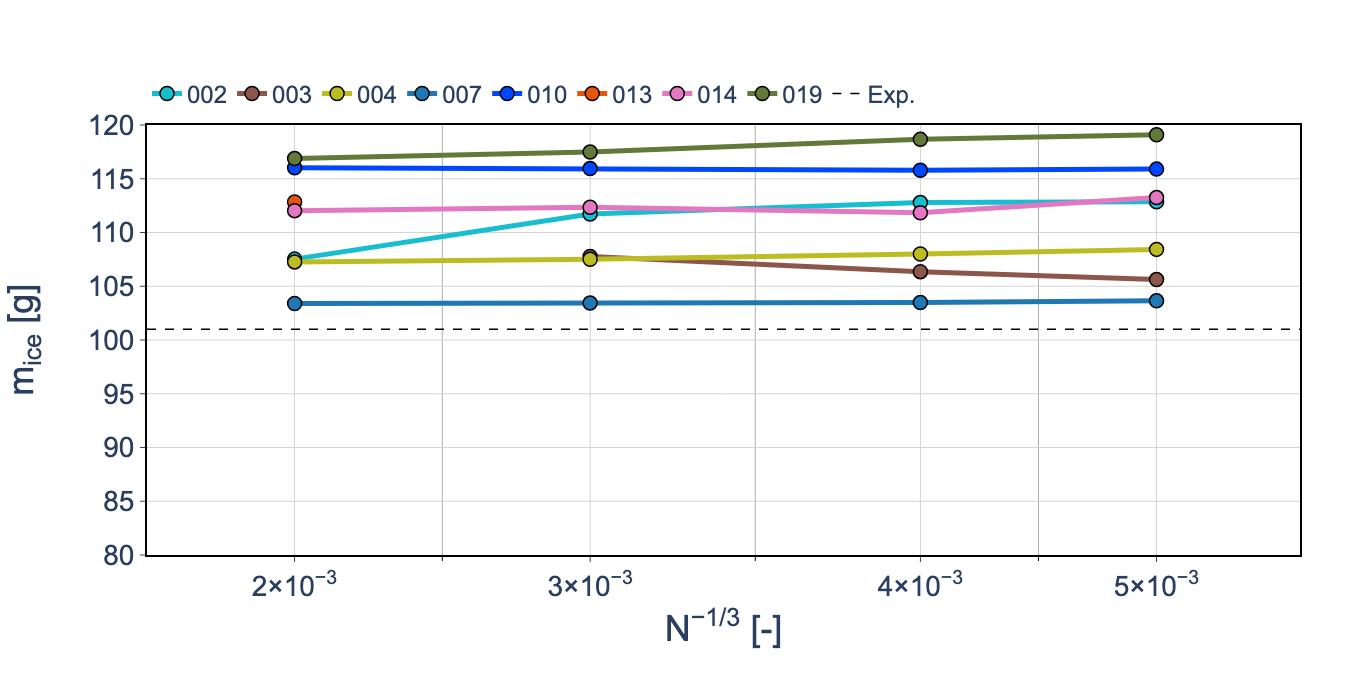
\includegraphics[trim={0cm 1cm 1cm 2.6cm}, clip, width=\textwidth]{FIGURES/ICE_ACCRETION/tc_naca0012_ae3932_ice_mass_vs_n_unspecified_bins15_all_grid_levels.png}
    {\scriptsize\textbf{AE3932}}
\end{column}

\begin{column}{0.50\textwidth}
    \centering
    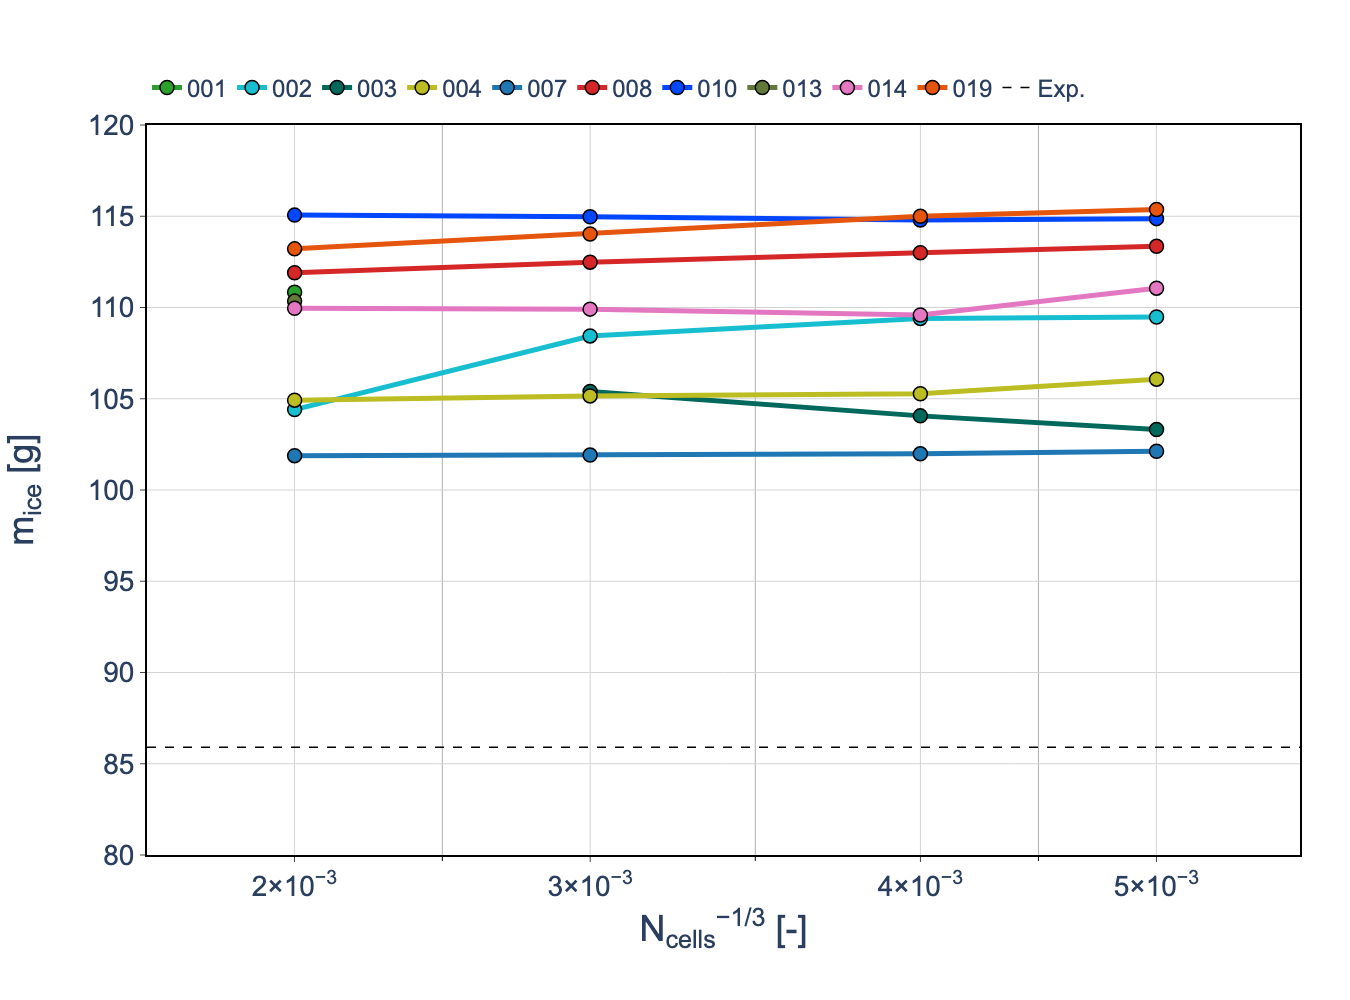
\includegraphics[trim={0cm 1cm 1cm 2.6cm}, clip, width=\textwidth]{FIGURES/ICE_ACCRETION/tc_naca0012_ae3933_ice_mass_vs_n_unspecified_bins15_all_grid_levels.png}
    {\scriptsize\textbf{AE3933}}
\end{column}

\end{columns}

\vspace{-0.15cm}

\begin{block}{\scriptsize Observations}
\begin{itemize}
    \item At L1, the median ice mass is approximately $110$ g for both conditions, with a relative IQR of about $7\%$.
    \item Grid sensitivity is limited for most submissions, with deviations generally remaining within approximately $5\%$ of L1.
    \item AE3933 predicts at most a $\sim3\%$ reduction in ice mass relative to AE3932, compared with $\sim15\%$ experimentally.
\end{itemize}
\end{block}

\end{frame}


% ============================================================
%  Ice Mass Droplet-Distribution Sensitivity
% ============================================================

\begin{frame}{\small  Ice Mass Sensitivity to Droplet Distribution (L1)}
\scriptsize

\begin{columns}[T,onlytextwidth]

\begin{column}{0.50\textwidth}
    \centering
    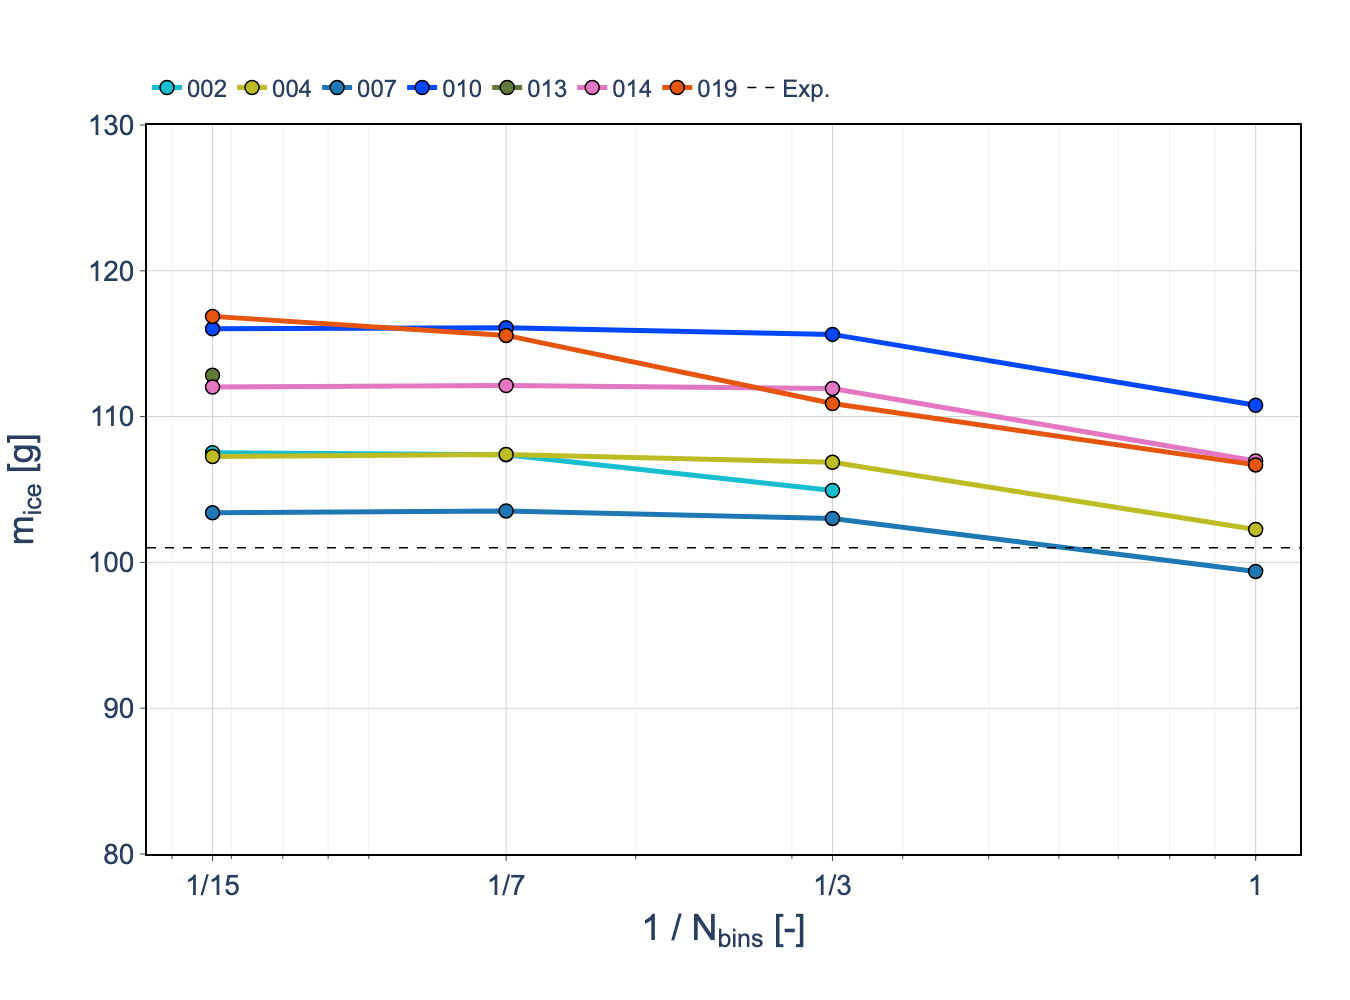
\includegraphics[trim={0cm 1cm 1cm 2.6cm}, clip, width=\textwidth]{FIGURES/ICE_ACCRETION/tc_naca0012_ae3932_ice_mass_vs_n_unspecified_l1_vs_inverse_bins.png}

    \vspace{0.05cm}

    {\scriptsize\textbf{AE3932}}
\end{column}

\begin{column}{0.50\textwidth}
    \centering
    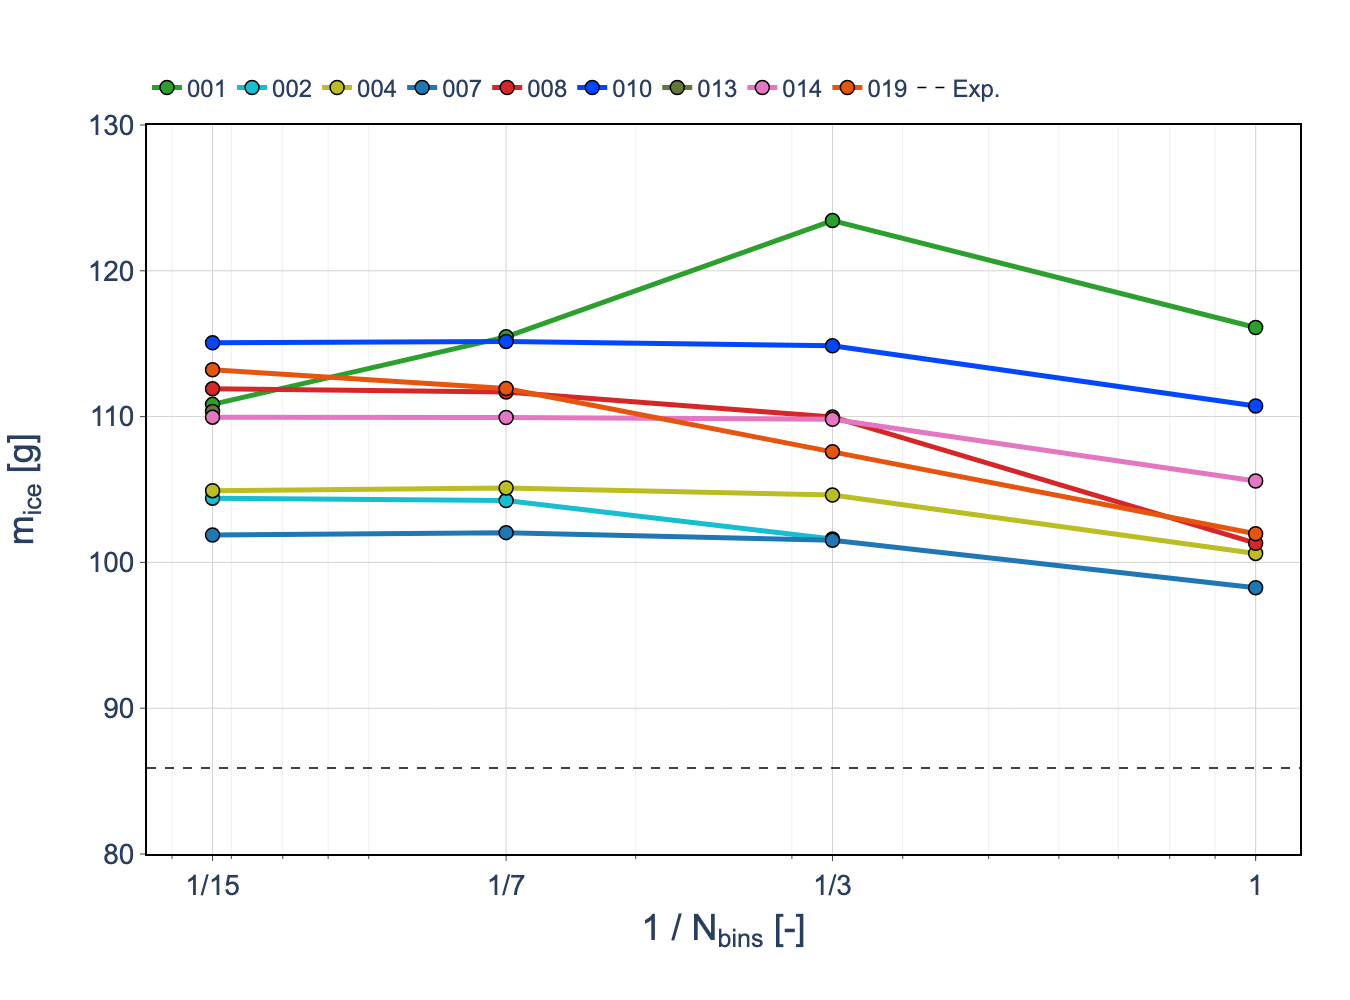
\includegraphics[trim={0cm 1cm 1cm 2.6cm}, clip, width=\textwidth]{FIGURES/ICE_ACCRETION/tc_naca0012_ae3933_ice_mass_vs_n_unspecified_l1_vs_inverse_bins.png}

    \vspace{0.05cm}

    {\scriptsize\textbf{AE3933}}
\end{column}

\end{columns}

\vspace{-0.15cm}

\begin{block}{\scriptsize Observations}
\begin{itemize}
    \item The 15- and 7-bin distributions produce comparable ice masses.
    \item Sensitivity increases for 3 bins and is greatest for the single-bin.
\end{itemize}
\end{block}

\end{frame}


% ============================================================
%  Ice-to-Water Mass Ratio
% ============================================================

\begin{frame}{\small  Ice-to-Water Mass Ratio}
\scriptsize

\vspace{-0.15cm}
\begin{columns}[T,onlytextwidth]

\begin{column}{0.50\textwidth}
    \centering
    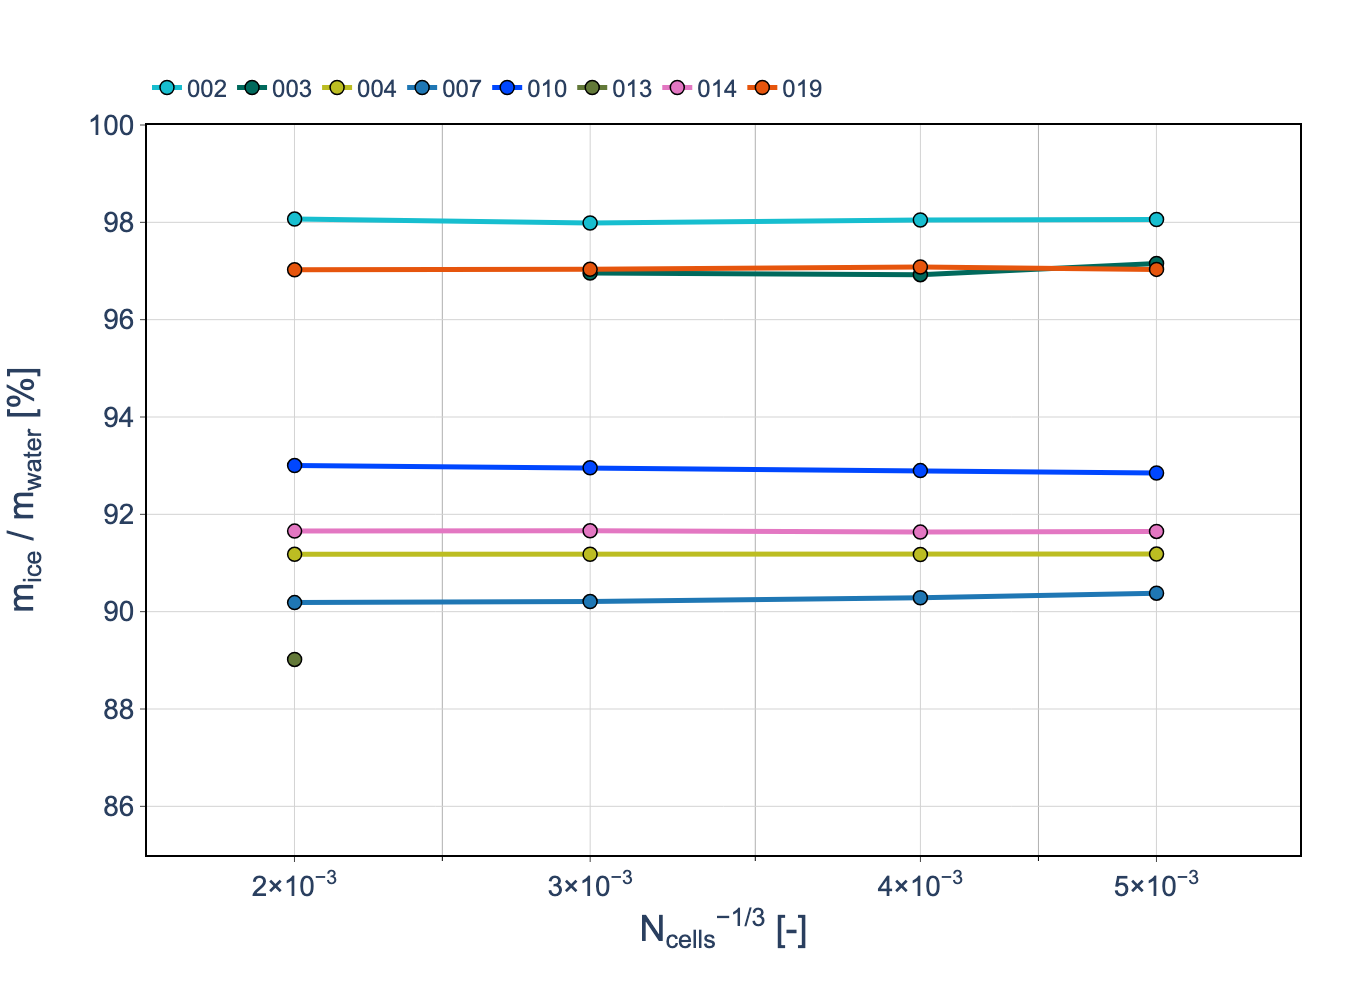
\includegraphics[trim={0cm 1cm 1cm 2.6cm}, clip, width=\textwidth]{FIGURES/ICE_ACCRETION/tc_naca0012_ae3932_ice_to_water_ratio_vs_n_required_bins15.png}

    \vspace{0.05cm}

    {\scriptsize\textbf{AE3932}}
\end{column}

\begin{column}{0.50\textwidth}
    \centering
    \IfFileExists{FIGURES/ICE_ACCRETION/tc_naca0012_ae3933_ice_to_water_ratio_vs_n_required_bins15.png}{%
        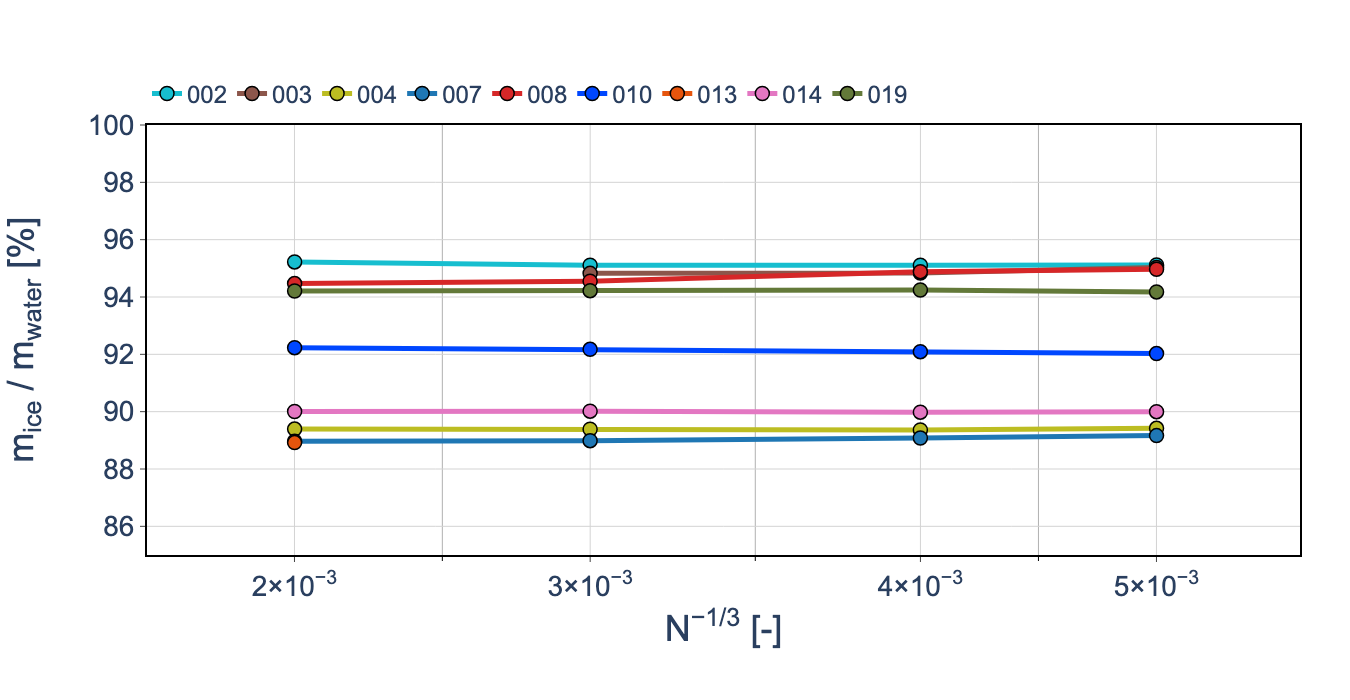
\includegraphics[trim={0cm 1cm 1cm 2.6cm}, clip, width=\textwidth]{FIGURES/ICE_ACCRETION/tc_naca0012_ae3933_ice_to_water_ratio_vs_n_required_bins15.png}%
    }{%
        \fbox{\parbox[c][0.27\textheight][c]{0.92\textwidth}{\centering
        \scriptsize AE3933 ice-to-water ratio figure unavailable}}%
    }

    \vspace{0.05cm}

    {\scriptsize\textbf{AE3933}}
\end{column}

\end{columns}

\vspace{-0.15cm}

\begin{block}{\scriptsize Observations}
\begin{itemize}
    \item Approximately $90-98\%$ of the impinged water is converted into ice for both conditions.
    \item AE3933 exhibits a lower ice-to-water ratio, indicating greater water loss.
    \item Including evaporation closes the mass balance to approximately $100\%$, identifying evaporation as the primary water-loss mechanism.
\end{itemize}
\end{block}

\end{frame}


% % ============================================================
% %  Ice and Evaporation-to-Water Mass Ratio
% % ============================================================

% \begin{frame}{\small  Ice and Evaporation-to-Water Mass Ratio}
% \scriptsize

% \begin{columns}[T,onlytextwidth]

% \begin{column}{0.50\textwidth}
%     \centering
%     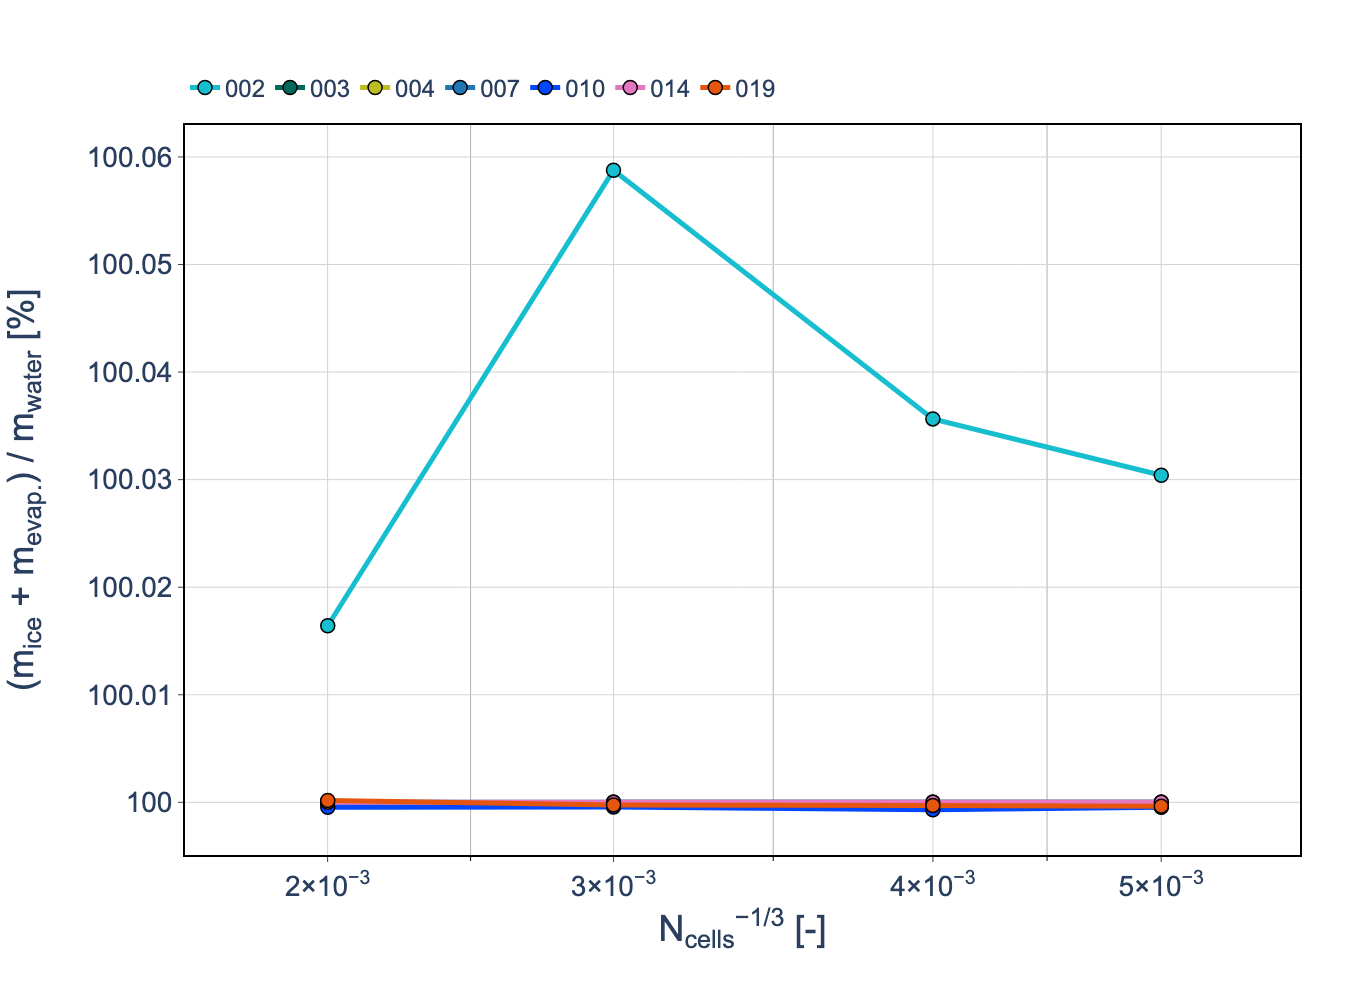
\includegraphics[width=\textwidth]{FIGURES/ICE_ACCRETION/tc_naca0012_ae3932_ice_evap_to_water_ratio_vs_n_required_bins15.png}

%     \vspace{0.05cm}

%     {\scriptsize\textbf{AE3932}}
% \end{column}

% \begin{column}{0.50\textwidth}
%     \centering
%     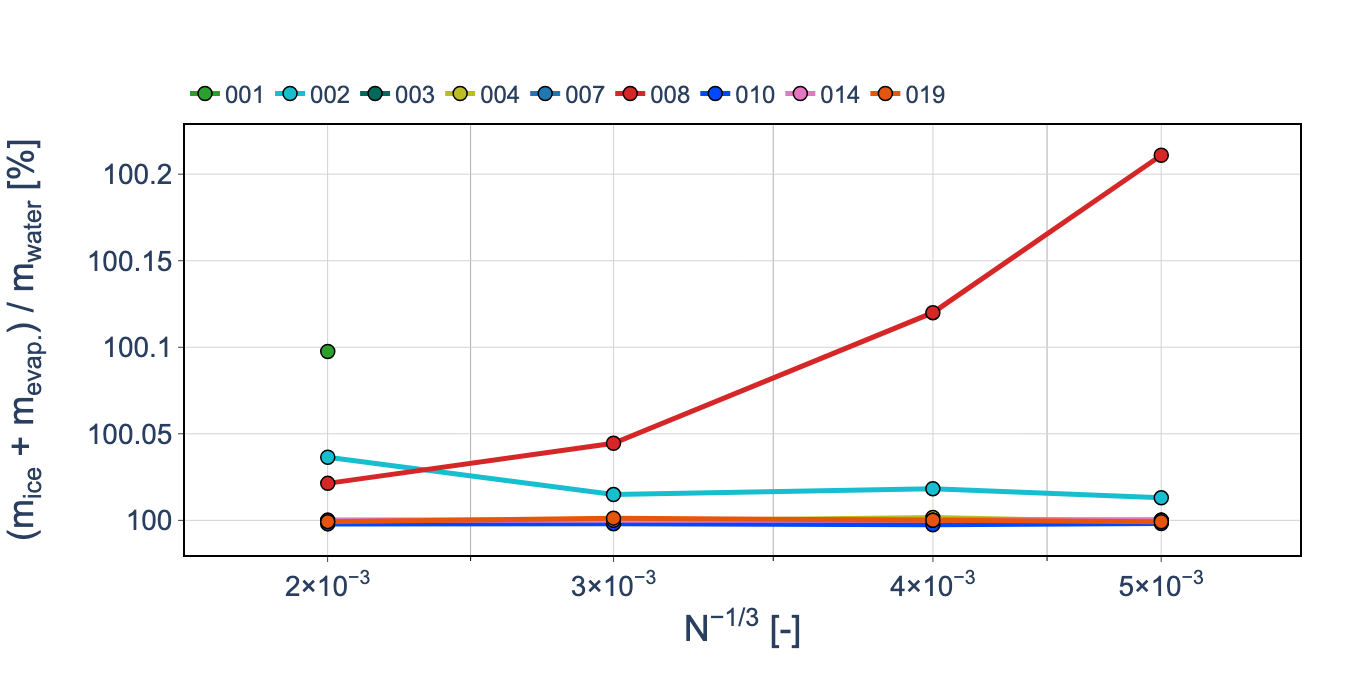
\includegraphics[width=\textwidth]{FIGURES/ICE_ACCRETION/tc_naca0012_ae3933_ice_evap_to_water_ratio_vs_n_required_bins15.png}

%     \vspace{0.05cm}

%     {\scriptsize\textbf{AE3933}}
% \end{column}

% \end{columns}

% \vspace{0.05cm}

% \begin{block}{\scriptsize Observations}
% \begin{itemize}
%     \item The combined ice and evaporated-water mass accounts for approximately $100\%$ of the impinged water for most submissions.
%     \item This indicates that the lower ice-to-water ratio for AE3933 is primarily associated with increased evaporation.
%     \item Values slightly above $100\%$ are observed for a few submissions and are likely attributable to numerical integration or round-off errors.
% \end{itemize}
% \end{block}

% \end{frame}

% ============================================================
%  Ice Shapes
% ============================================================

\begin{frame}{\small  Ice Shapes (L2, 15 Bins)}
\scriptsize
\vspace{-0.15cm}
% ------------------------------------------------------------
% Experimental ice shapes
% ------------------------------------------------------------

\only<1>{
\begin{columns}[T,onlytextwidth]

\begin{column}{0.50\textwidth}
    \centering
    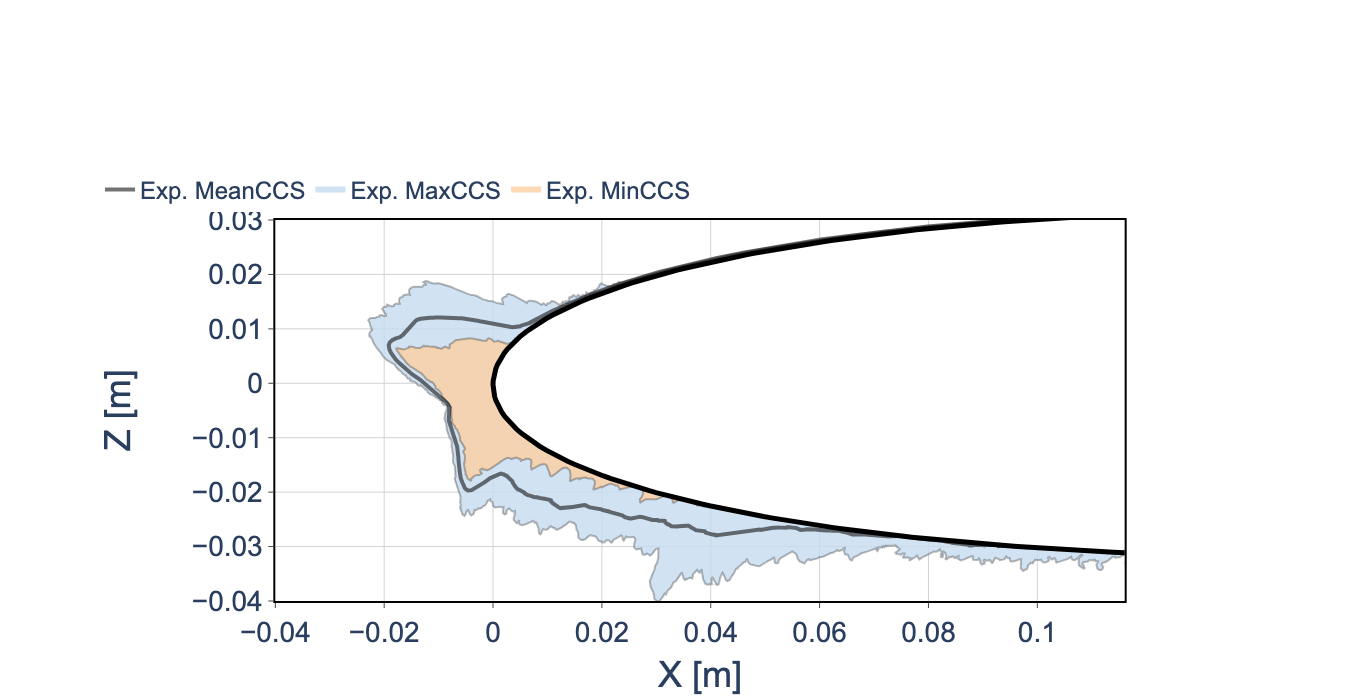
\includegraphics[width=\textwidth]{FIGURES/ICE_SHAPES/tc_naca0012_ae3932_experimental_ice_shape.png}

    \vspace{0.05cm}

    {\scriptsize\textbf{AE3932 -- Experiment}}
\end{column}

\begin{column}{0.50\textwidth}
    \centering
    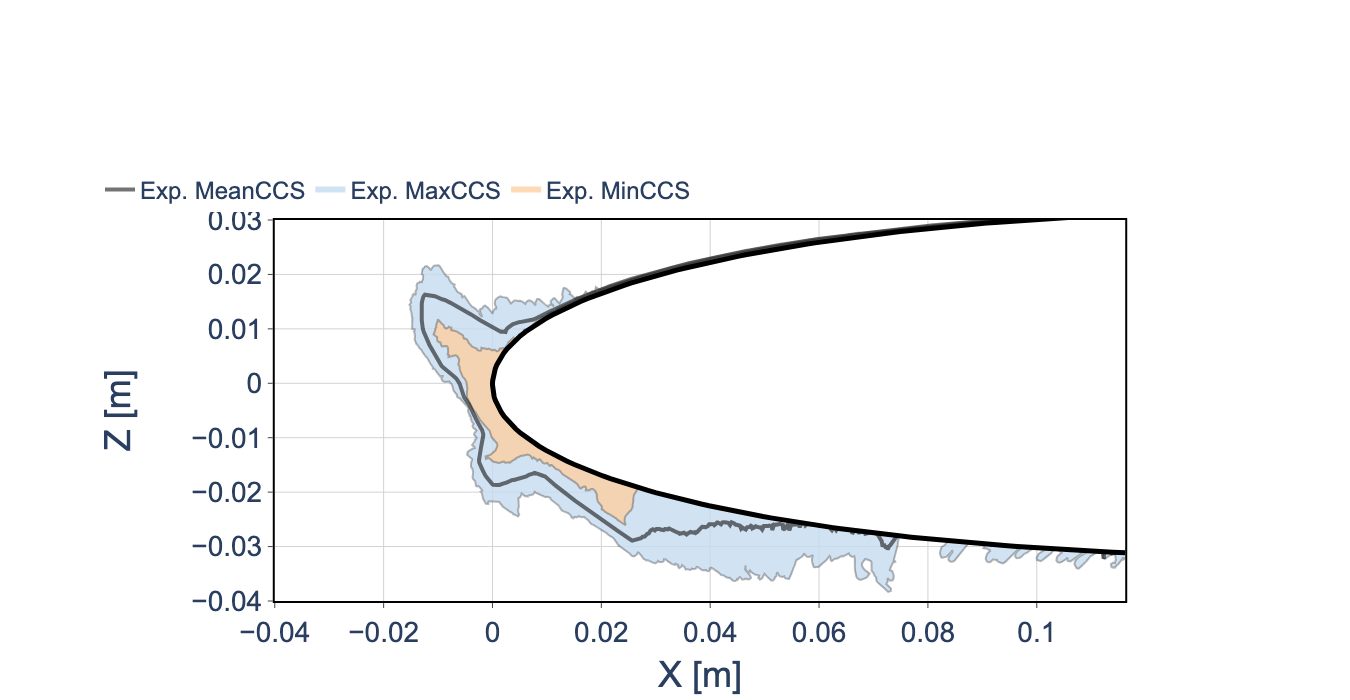
\includegraphics[width=\textwidth]{FIGURES/ICE_SHAPES/tc_naca0012_ae3933_experimental_ice_shape.png}

    \vspace{0.05cm}

    {\scriptsize\textbf{AE3933 -- Experiment}}
\end{column}

\end{columns}
}

% ------------------------------------------------------------
% Standard ice-shape comparison
% ------------------------------------------------------------

\only<2>{
\begin{columns}[T,onlytextwidth]

\begin{column}{0.50\textwidth}
    \centering
    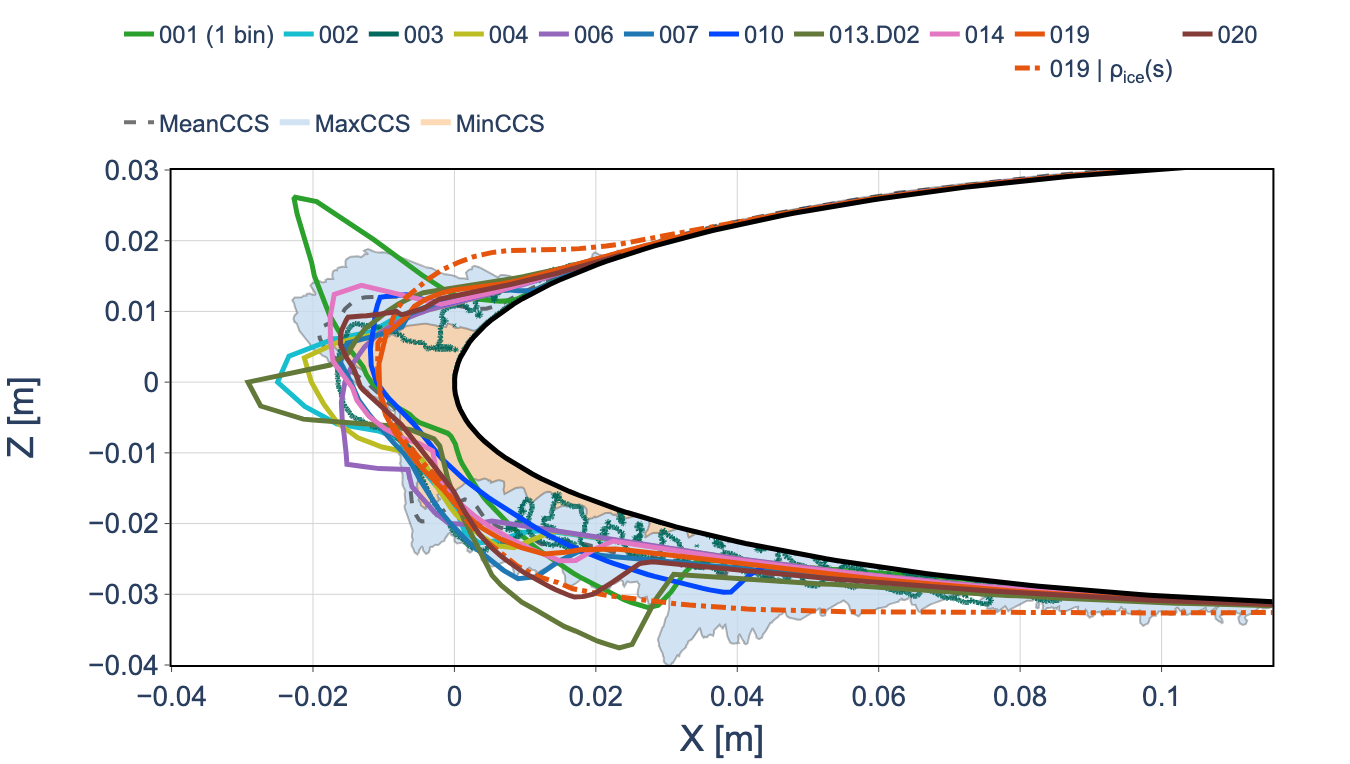
\includegraphics[width=\textwidth]{FIGURES/ICE_SHAPES/tc_naca0012_ae3932_L2_single_layer_ice_shape_slice_0p9144_bins15_roughness_unspecified.png}

    \vspace{0.05cm}

    {\scriptsize\textbf{AE3932}}
\end{column}

\begin{column}{0.50\textwidth}
    \centering
    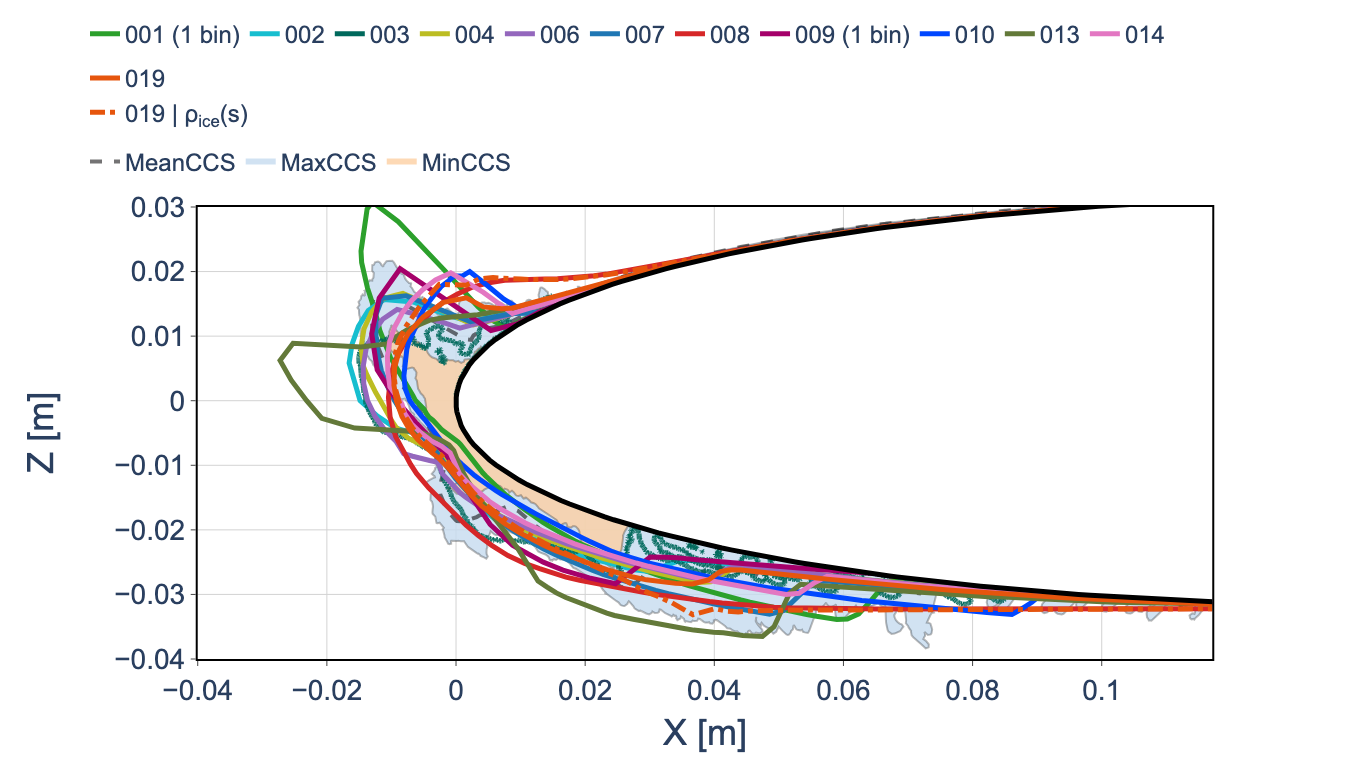
\includegraphics[width=\textwidth]{FIGURES/ICE_SHAPES/tc_naca0012_ae3933_L2_single_layer_ice_shape_slice_0p9144_bins15_roughness_unspecified.png}

    \vspace{0.05cm}

    {\scriptsize\textbf{AE3933}}
\end{column}

\end{columns}
}

% ------------------------------------------------------------
% Ice shapes grouped by roughness
% ------------------------------------------------------------

\only<3>{
\begin{columns}[T,onlytextwidth]

\begin{column}{0.50\textwidth}
    \centering
    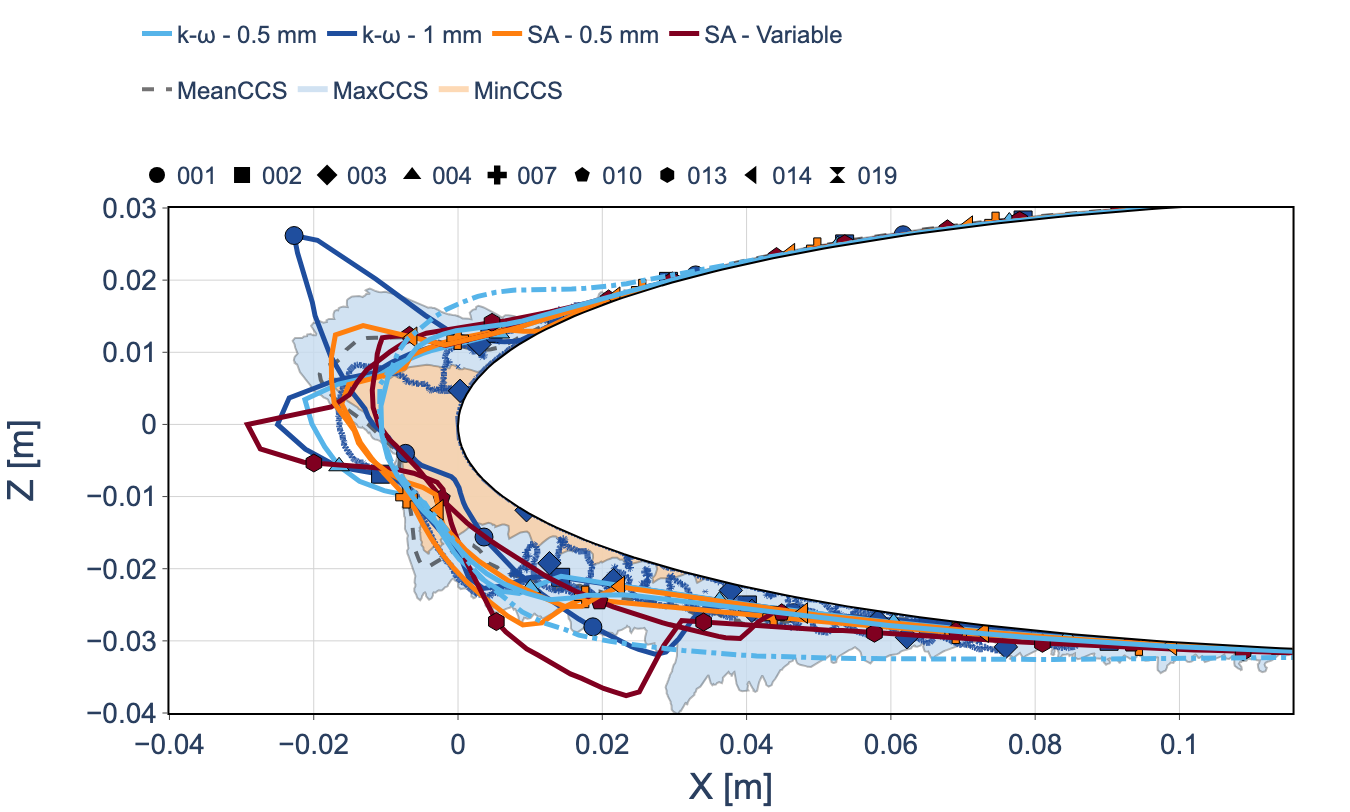
\includegraphics[width=\textwidth]{FIGURES/ICE_SHAPES/tc_naca0012_ae3932_L2_single_layer_ice_shape_slice_0p9144_bins15_grouped_turbulence_models.png}

    \vspace{0.05cm}

    {\scriptsize\textbf{AE3932}}
\end{column}

\begin{column}{0.50\textwidth}
    \centering
    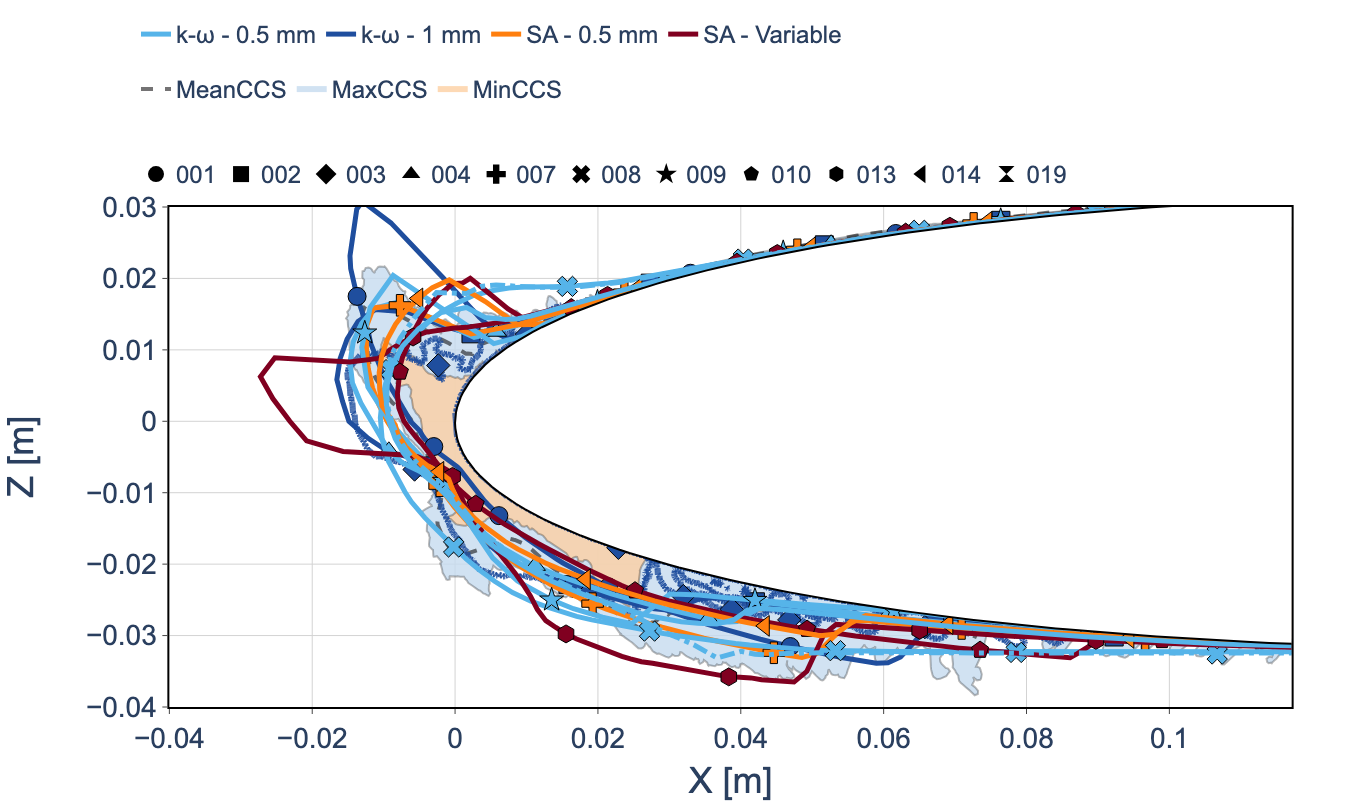
\includegraphics[width=\textwidth]{FIGURES/ICE_SHAPES/tc_naca0012_ae3933_L2_single_layer_ice_shape_slice_0p9144_bins15_grouped_turbulence_models.png}

    \vspace{0.05cm}

    {\scriptsize\textbf{AE3933}}
\end{column}

\end{columns}

\vspace{-0.1cm}
\centering
\textbf{Grouped by Turbulence Model / Roughness}
}

\begin{block}{\scriptsize Observations}
\begin{itemize}
    \item<1-> Experiments show a clear difference in ice shape, particularly in upper-horn orientation.
    \item<2-> Code-to-code variability is reflected in the predicted ice shapes and horn angles.
    \item<2-> The experimental difference between conditions is reproduced to varying degrees.
    \item<3-> Horn orientation is influenced by turbulence modeling and roughness height, with the geometry-extrusion method playing a major role.
\end{itemize}
\end{block}

\end{frame}

% ============================================================
%  Ice-Shape Roughness Effects
% ============================================================

\begin{frame}{\small Ice Shapes (L2, 15 Bins)}
\scriptsize
\centering

% ------------------------------------------------------------
% AE3932
% ------------------------------------------------------------
% {\scriptsize\textbf{AE3932}}
% \vspace{-0.25cm}

% 
\includegraphics[trim={0cm 2.cm 1cm 1.0cm}, clip, width=.8\textwidth]{%
% FIGURES/ICE_SHAPES/tc_naca0012_ae3932_L2_single_layer_ice_shape_slice_0p9144_bins15_grouped_turbulence_models_panels.png}

\begin{tikzpicture}
    % Figure
    \node[inner sep=0] (fig) {
        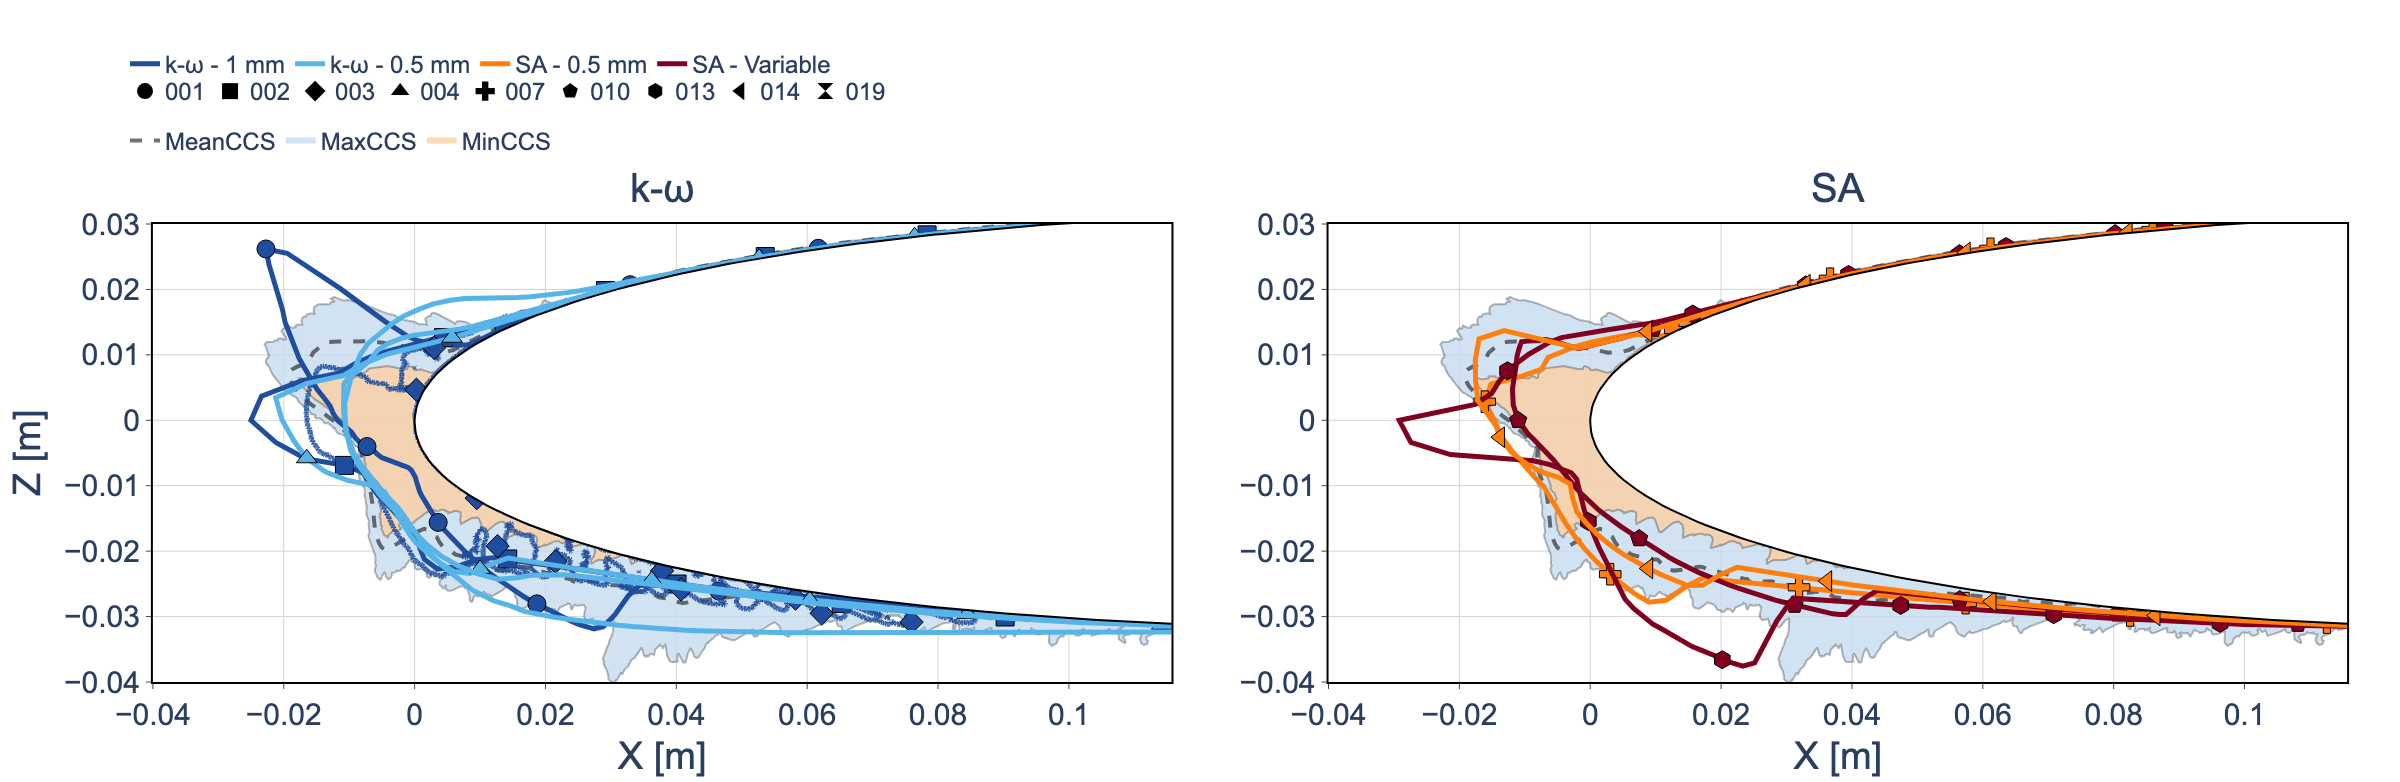
\includegraphics[
            trim={0cm 2cm 1cm 1.0cm},
            clip,
            width=.8\textwidth
        ]{FIGURES/ICE_SHAPES/tc_naca0012_ae3932_L2_single_layer_ice_shape_slice_0p9144_bins15_grouped_turbulence_models_panels.png}
    };

    % Text ON TOP of figure
    \node[
        anchor=north,
        fill=white,
        inner sep=1pt
    ] at ([yshift=-5mm]fig.north)
    {\scriptsize\textbf{AE3932}};
\end{tikzpicture}

% ------------------------------------------------------------
% AE3933
% ------------------------------------------------------------
{\scriptsize\textbf{AE3933}}


\includegraphics[trim={0cm 0cm 1cm 7.cm}, clip, width=.8\textwidth]{%
FIGURES/ICE_SHAPES/tc_naca0012_ae3933_L2_single_layer_ice_shape_slice_0p9144_bins15_grouped_turbulence_models_panels.png}
\end{frame}

% ============================================================
% Experimental Upper Horn Angle
% ============================================================

\begin{frame}{\small Experimental Upper Horn Angle}
\scriptsize

\vspace{-0.25cm}

% ------------------------------------------------------------
% AE3932
% ------------------------------------------------------------

\centering
\textbf{AE3932}

\vspace{0.03cm}

\begin{minipage}[t]{0.25\textwidth}
    \centering
    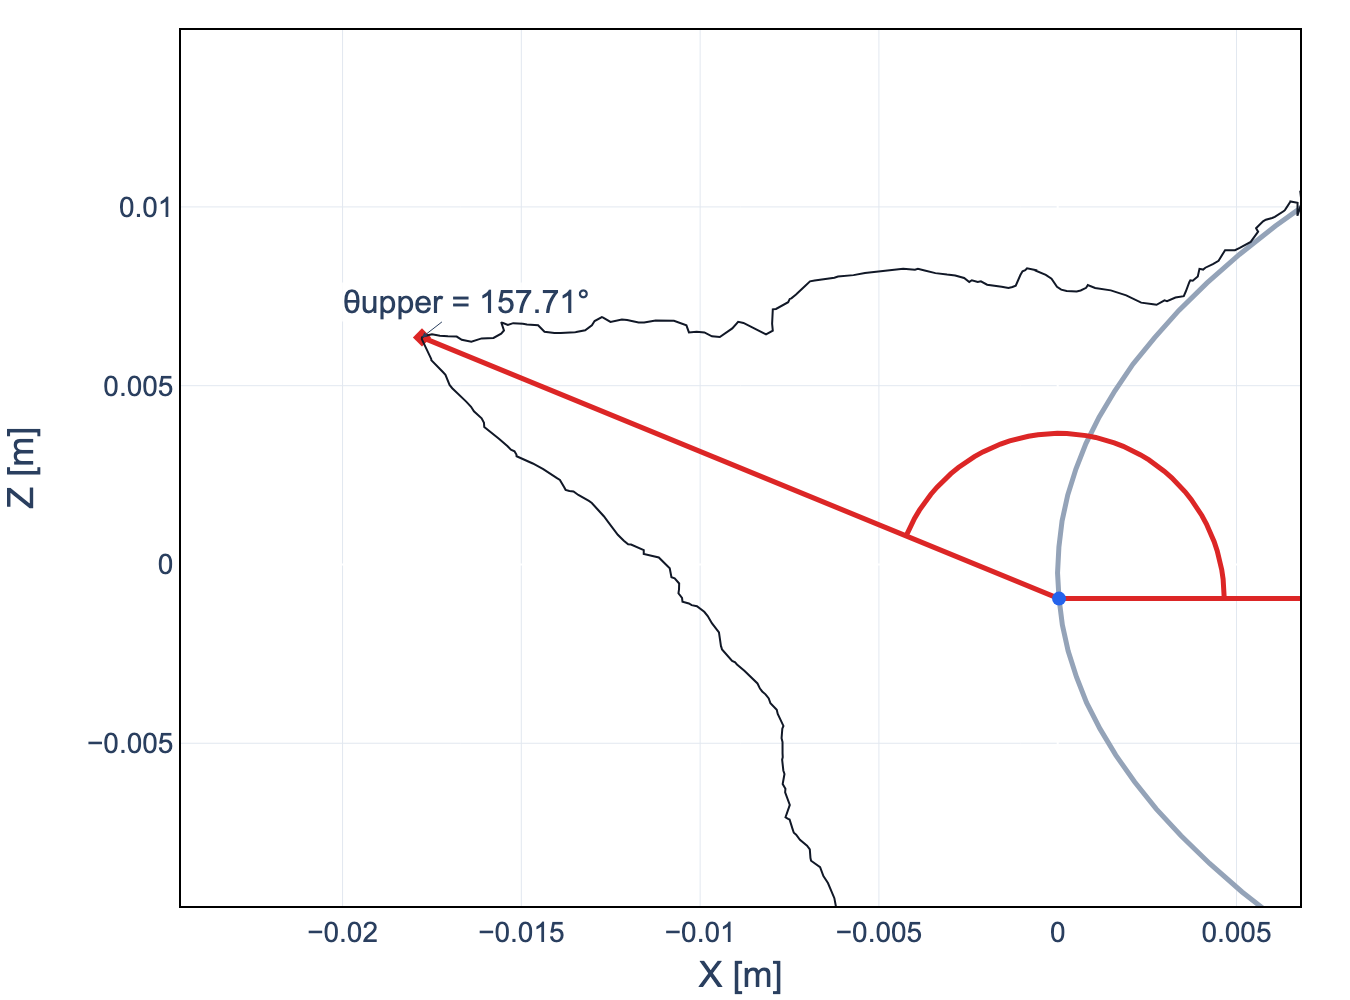
\includegraphics[
        trim={0cm 0cm 1cm 0.6cm},
        clip,
        width=\textwidth
    ]{FIGURES/ICE_HORNS/tc_naca0012_ae3932_minccs_upper_horn_angle_method.png}
\end{minipage}
\hspace{0.01\textwidth}
\begin{minipage}[t]{0.25\textwidth}
    \centering
    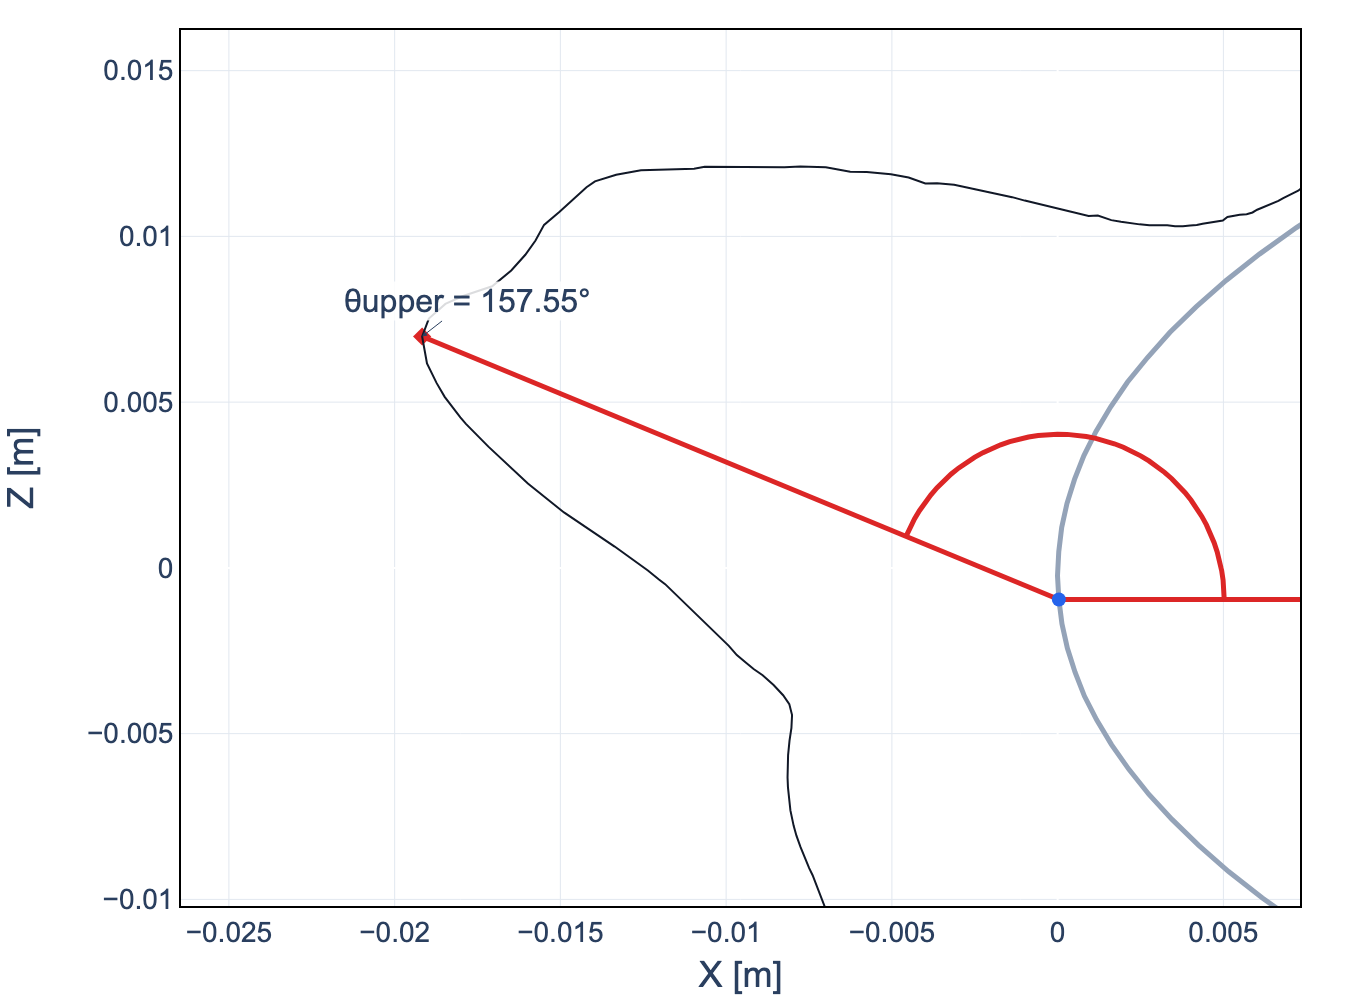
\includegraphics[
        trim={0cm 0cm 1cm 0.6cm},
        clip,
        width=\textwidth
    ]{FIGURES/ICE_HORNS/tc_naca0012_ae3932_meanccs_upper_horn_angle_method.png}
\end{minipage}
\hspace{0.01\textwidth}
\begin{minipage}[t]{0.25\textwidth}
    \centering
    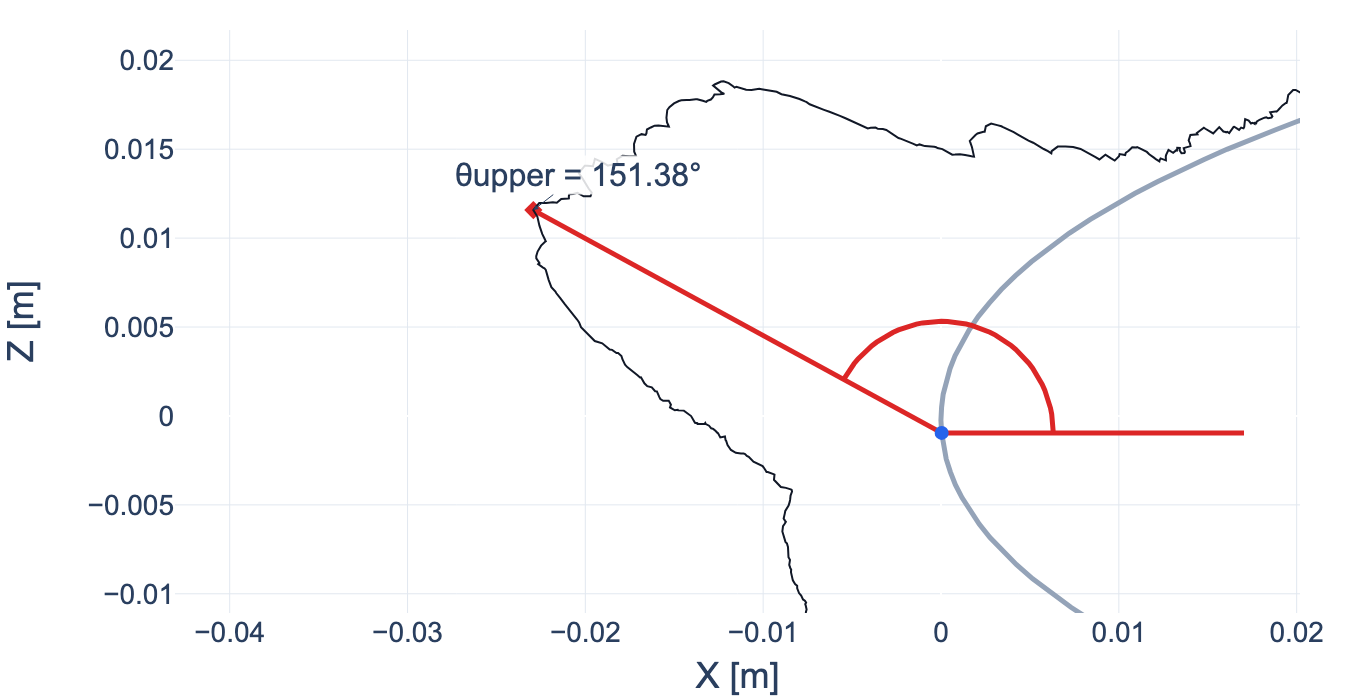
\includegraphics[
        trim={0cm 0cm 1cm 0.6cm},
        clip,
        width=\textwidth
    ]{FIGURES/ICE_HORNS/tc_naca0012_ae3932_maxccs_upper_horn_angle_method.png}
\end{minipage}



% ------------------------------------------------------------
% AE3933
% ------------------------------------------------------------

\centering
\textbf{AE3933}

\vspace{0.03cm}

\begin{minipage}[t]{0.25\textwidth}
    \centering
    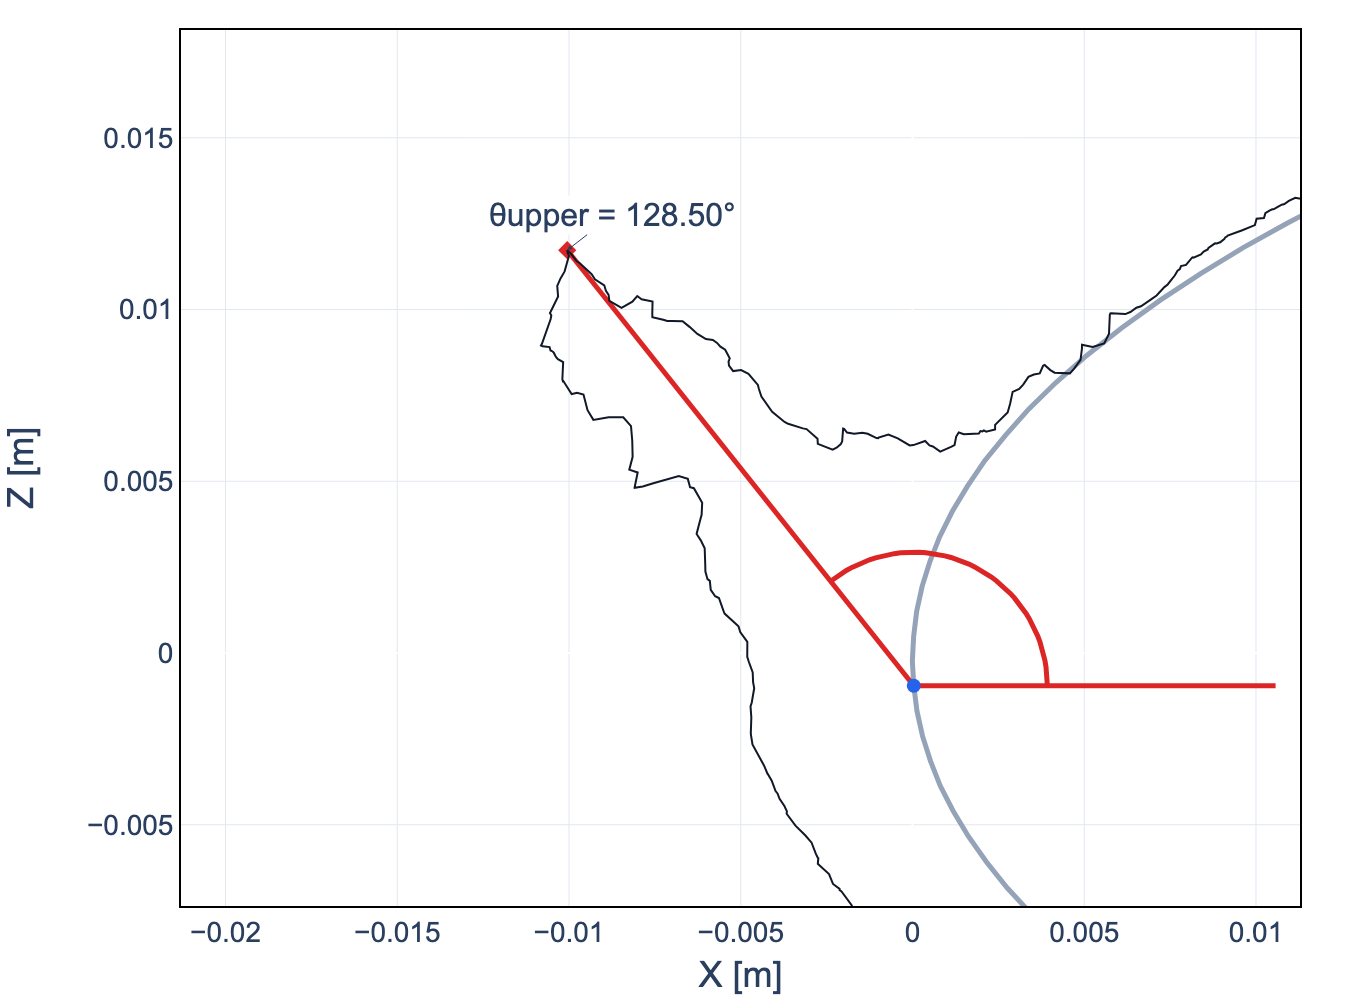
\includegraphics[
        trim={0cm 0cm 1cm 0.6cm},
        clip,
        width=\textwidth
    ]{FIGURES/ICE_HORNS/tc_naca0012_ae3933_minccs_upper_horn_angle_method.png}

    \vspace{-0.08cm}
    \textbf{MinCCS}
\end{minipage}
\hspace{0.01\textwidth}
\begin{minipage}[t]{0.25\textwidth}
    \centering
    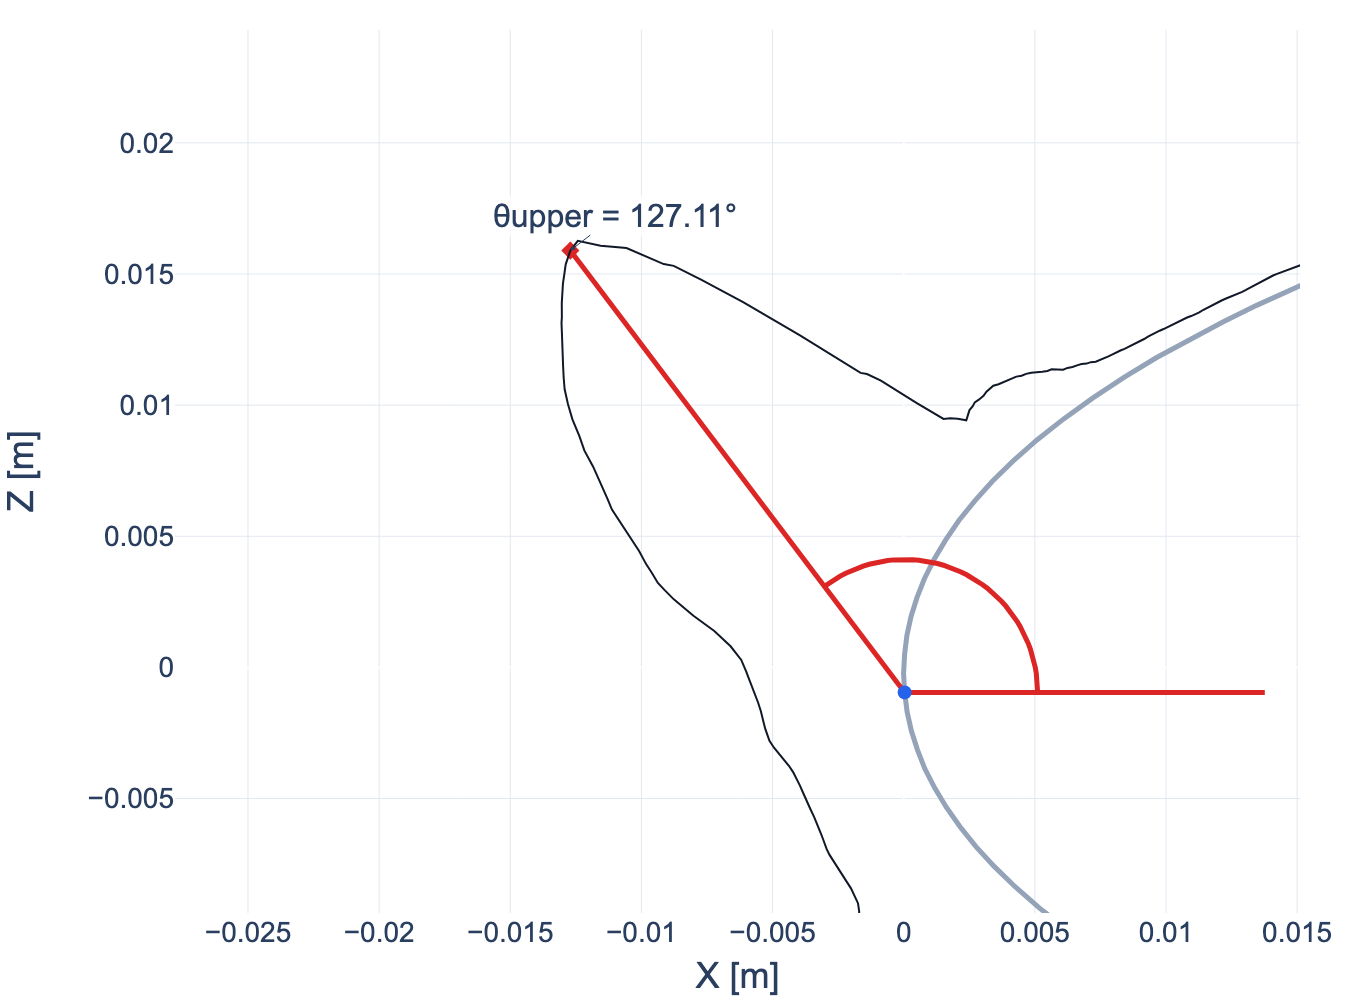
\includegraphics[
        trim={0cm 0cm 1cm 0.6cm},
        clip,
        width=\textwidth
    ]{FIGURES/ICE_HORNS/tc_naca0012_ae3933_meanccs_upper_horn_angle_method.png}

    \vspace{-0.08cm}
    \textbf{MeanCCS}
\end{minipage}
\hspace{0.01\textwidth}
\begin{minipage}[t]{0.25\textwidth}
    \centering
    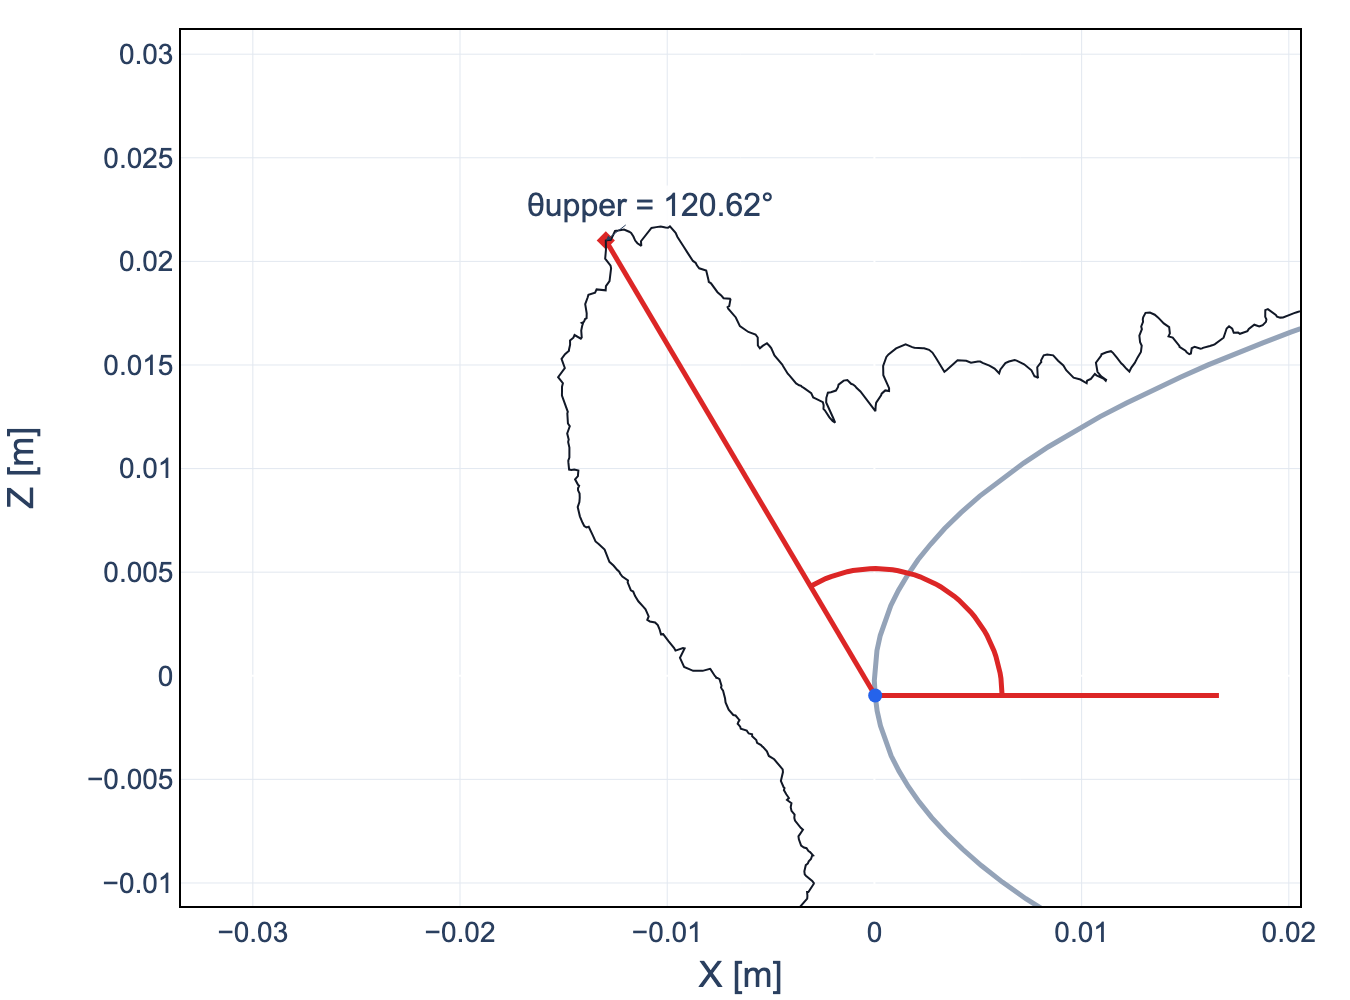
\includegraphics[
        trim={0cm 0cm 1cm 0.6cm},
        clip,
        width=\textwidth
    ]{FIGURES/ICE_HORNS/tc_naca0012_ae3933_maxccs_upper_horn_angle_method.png}

    \vspace{-0.08cm}
    \textbf{MaxCCS}
\end{minipage}

% ------------------------------------------------------------
% Experimental reference
% ------------------------------------------------------------

\begin{block}{\scriptsize Experimental Reference}
\begin{itemize}
    \item The experimental upper-horn angle ranges from approximately
    $151$--$158^\circ$ for AE3932 and $121$--$129^\circ$ for AE3933.
\end{itemize}
\end{block}

\end{frame}


% ============================================================
%  Upper Horn Angle Grid Convergence
% ============================================================

\begin{frame}{\small  Upper Horn Angle Grid Convergence (15 Bins)}
\scriptsize
\vspace{-0.15cm}
\begin{columns}[T,onlytextwidth]

\begin{column}{0.50\textwidth}
    \centering
    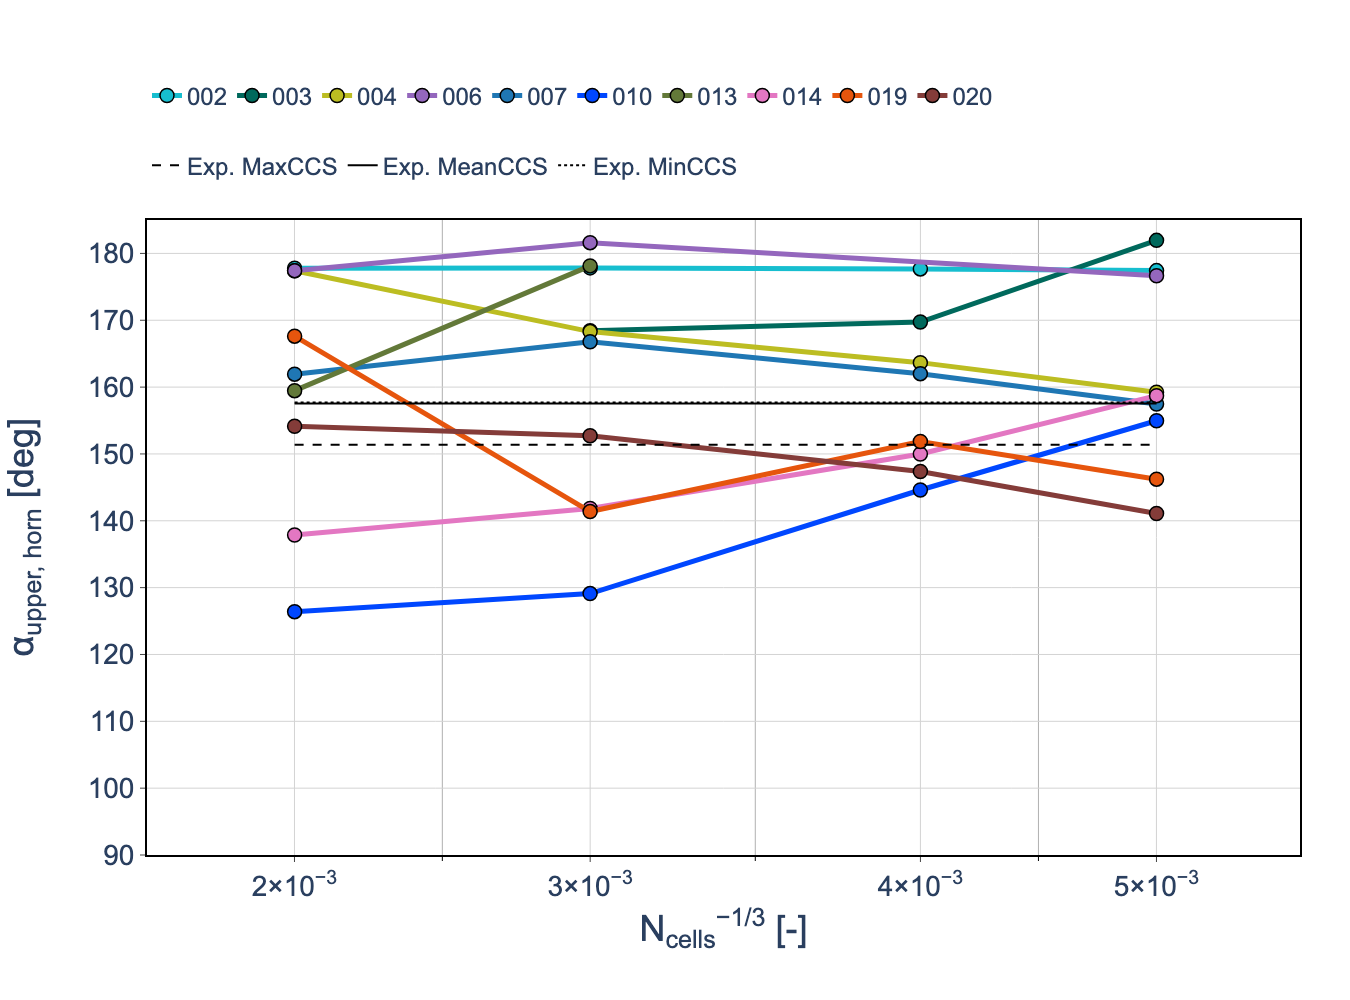
\includegraphics[trim={0cm 1cm 1cm 2.6cm}, clip, width=\textwidth]{FIGURES/ICE_ACCRETION/tc_naca0012_ae3932_upper_horn_angle_bins15.png}

    \vspace{0.05cm}

    {\scriptsize\textbf{AE3932}}
\end{column}

\begin{column}{0.50\textwidth}
    \centering
    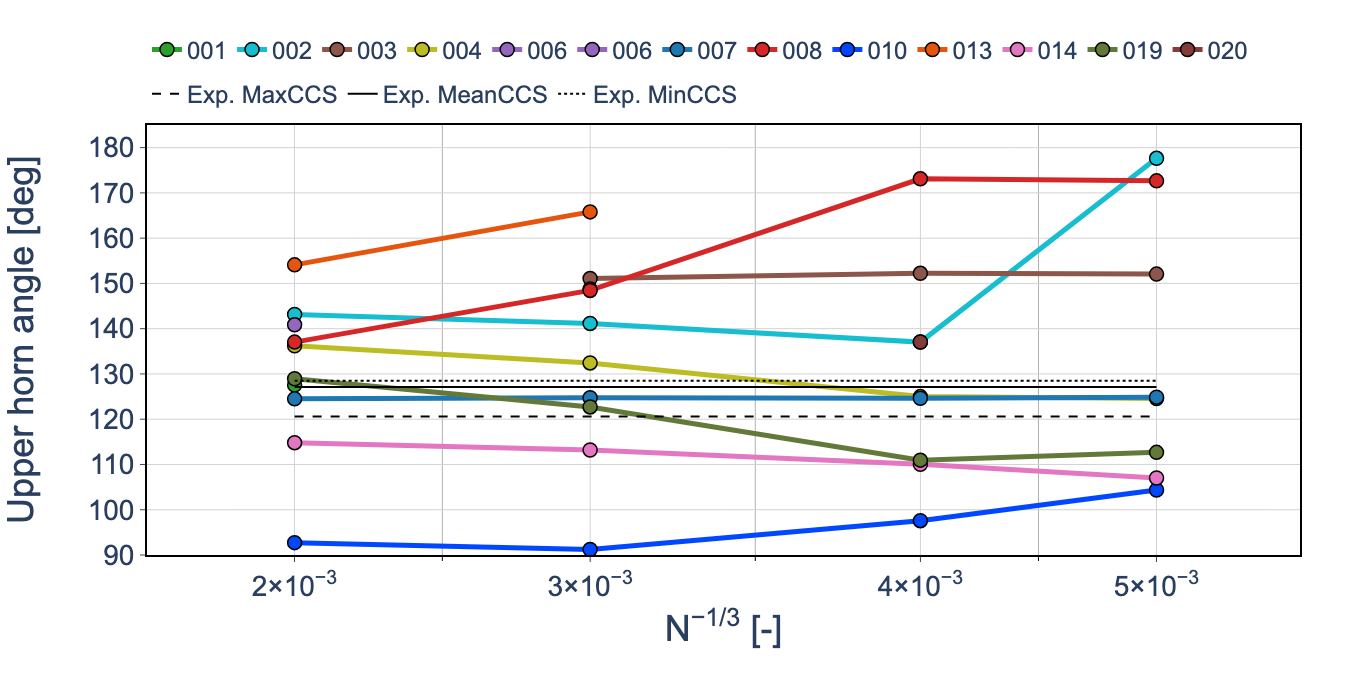
\includegraphics[trim={0cm 1cm 1cm 2.6cm}, clip, width=\textwidth]{FIGURES/ICE_ACCRETION/tc_naca0012_ae3933_upper_horn_angle_bins15.png}

    \vspace{0.05cm}

    {\scriptsize\textbf{AE3933}}
\end{column}

\end{columns}

\vspace{-0.15cm}

\begin{block}{\scriptsize Observations}
\begin{itemize}
    \item Horn-angle variability reflects the code-to-code scatter observed in the ice shapes.
    \item AE3933 predicts smaller upper-horn angles than AE3932, consistent with experiment.
    \item L1 scatter is comparable between conditions ($\mathrm{IQR}\approx16\%$ and $13\%$).
\end{itemize}
\end{block}

\end{frame}


% ============================================================
%  Upper Horn Angle Distribution Sensitivity
% ============================================================

\begin{frame}{\small  Upper Horn Angle Sensitivity to Droplet Distribution (L1)}
\scriptsize

\begin{columns}[T,onlytextwidth]

\begin{column}{0.50\textwidth}
    \centering
    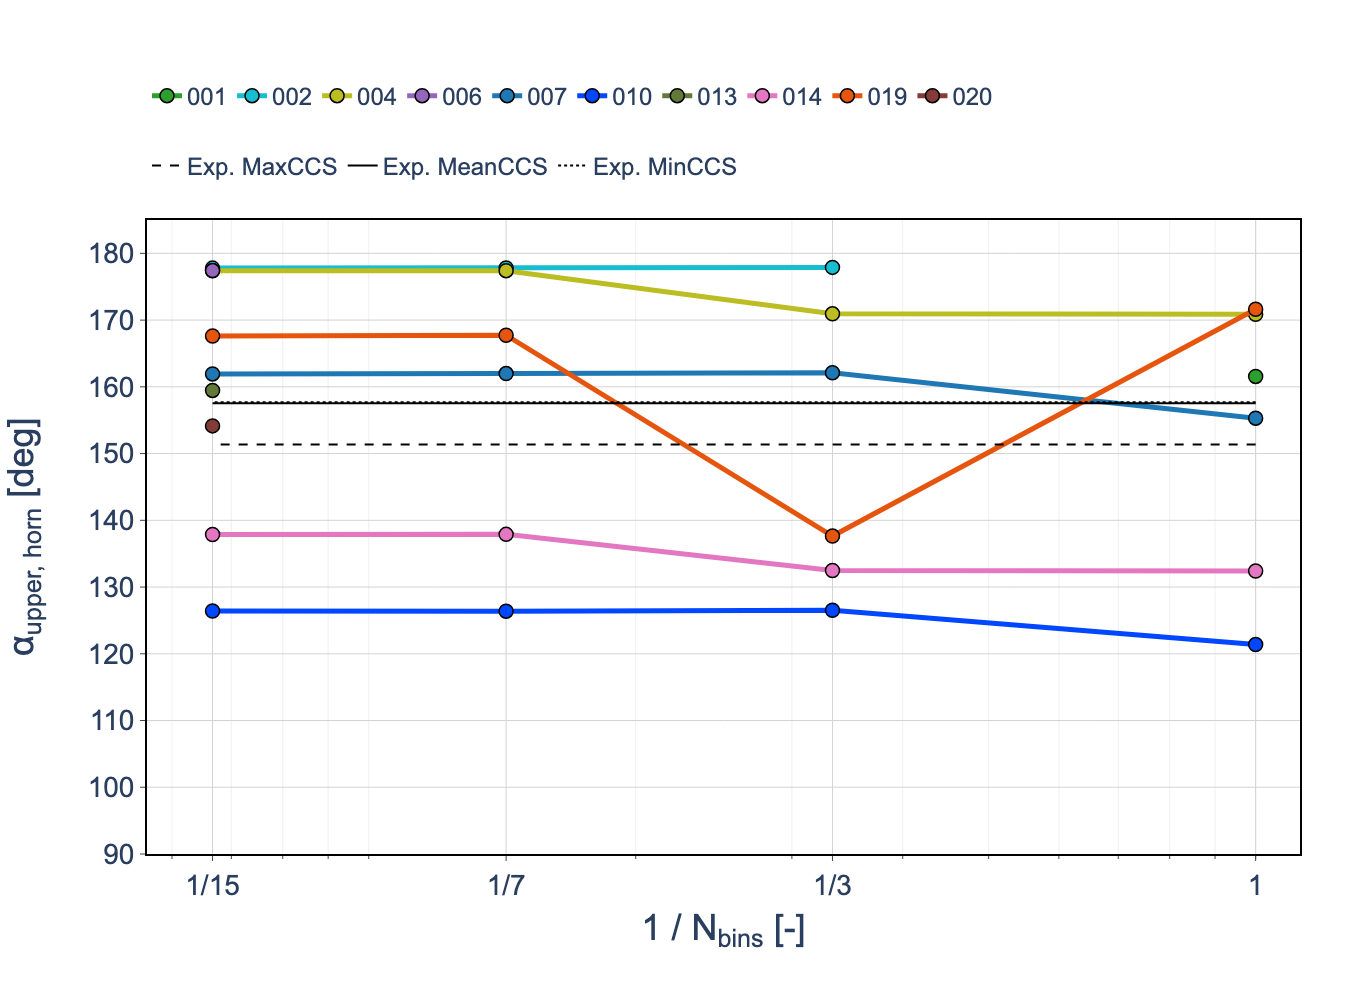
\includegraphics[trim={0cm 1cm 1cm 2.6cm}, clip, width=\textwidth]{FIGURES/ICE_ACCRETION/tc_naca0012_ae3932_upper_horn_angle_distribution_convergence_l1.png}

    \vspace{0.05cm}

    {\scriptsize\textbf{AE3932}}
\end{column}

\begin{column}{0.50\textwidth}
    \centering
    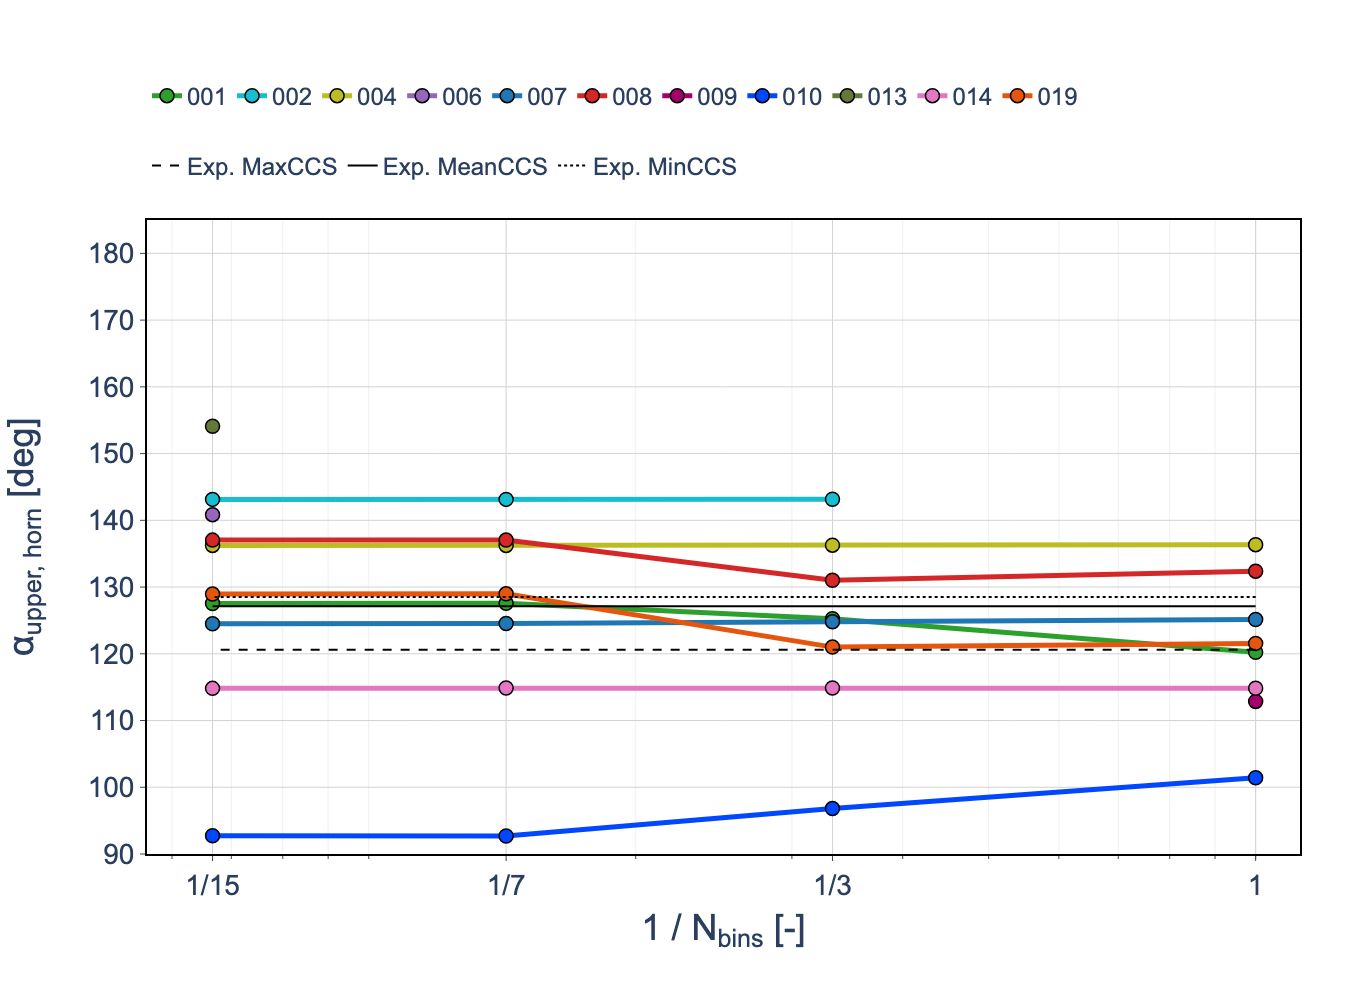
\includegraphics[trim={0cm 1cm 1cm 2.6cm}, clip, width=\textwidth]{FIGURES/ICE_ACCRETION/tc_naca0012_ae3933_upper_horn_angle_distribution_convergence_l1.png}

    \vspace{0.05cm}

    {\scriptsize\textbf{AE3933}}
\end{column}

\end{columns}

\vspace{0.15cm}

\begin{block}{\scriptsize Observations}
\begin{itemize}
    \item Upper-horn angle shows limited sensitivity to droplet-size discretization.
\end{itemize}
\end{block}

\end{frame}


% ============================================================
% Ice Accretion Assessment
% ============================================================

\begin{frame}{\small Ice Accretion Assessment}
\scriptsize

\begin{alertblock}{\scriptsize Ice Accretion Assessment}

\textbf{Ice-Mass Prediction}
\begin{itemize}
    \item Ice mass shows limited grid sensitivity, with 15- and 7-bin distributions producing comparable results.
    
    \item Approximately $90\%$ of the impinged water is converted into ice, with evaporation accounting for most of the remaining water mass.
\end{itemize}

\vspace{0.10cm}

\textbf{Response to Icing Condition}
\begin{itemize}
    \item AE3933 predicts less ice than AE3932, but substantially underestimates the experimental $\sim15\%$ reduction.
    
    \item The smaller AE3933 upper-horn angle is consistently captured, in agreement with the experimental trend.
\end{itemize}

\vspace{0.10cm}

\textbf{Ice-Shape Prediction}
\begin{itemize}
    \item Horn-angle variability reflects the code-to-code scatter observed in the ice shapes.
    
    \item Horn orientation is influenced not only by turbulence modeling and roughness height, but also by the geometry-extrusion method, which plays a major role.
    
    \item Horn angle shows limited sensitivity to droplet-size discretization.
\end{itemize}

\end{alertblock}

\end{frame}